\documentclass[letterpaper,13pt]{book}
\usepackage[spanish]{babel}
\addto\captionsspanish{
        \def\listtablename{\'Indice de tablas}%
        \def\tablename{Tabla}} 
\usepackage{graphicx, color}
\usepackage{amsmath}
\usepackage{amscd}
%\usepackage{youngtab}
\usepackage{titlesec}
\usepackage[latin1]{inputenc}
\usepackage{listings}
\usepackage{enumerate}
\usepackage{amssymb}
\usepackage{amsthm}
\usepackage{syntonly}
\usepackage{fancyhdr}
\usepackage{verbatim}
\usepackage{fancyvrb}


%***************************** Formato*********************************************
\newcommand{\bigrule}{\titlerule[0.5mm]}
\titleformat{\chapter}[display] % cambiamos el formato de los cap\'{\i}tulos
{\bfseries\Huge} % por defecto se usar\'{a}n caracteres de tama\~{n}o \Huge en negrita
{% contenido de la etiqueta
\titlerule % l\'{\i}nea horizontal
\filleft % texto alineado a la derecha
\Large\chaptertitlename\ % "Cap\'{\i}tulo" o "Ap\'{e}ndice" en tama\~{n}o \Large en lugar de \Huge
\Large\thechapter} % n\'{u}mero de cap\'{\i}tulo en tama\~{n}o \Large
{0mm} % espacio m\'{\i}nimo entre etiqueta y cuerpo
{\filleft} % texto del cuerpo alineado a la derecha
[\vspace{0.5mm} \bigrule] % despu\'{e}s del cuerpo, dejar espacio vertical y trazar l\'{\i}nea horizontal gruesa

\usepackage{fancyhdr}
\pagestyle{fancy}
\fancyhf{}
\fancyhead[LO]{\leftmark} % En las p\'{a}ginas impares, parte izquierda del encabezado, aparecer\'{a} el nombre de cap\'{\i}tulo
\fancyhead[RE]{\rightmark} % En las p\'{a}ginas pares, parte derecha del encabezado, aparecer\'{a} el nombre de secci\'{o}n
\fancyhead[RO,LE]{\thepage} % N\'{u}meros de p\'{a}gina en las esquinas de los encabezados

\renewcommand{\chaptermark}[1]{\markboth{\textbf{\thechapter. #1}}{}} % Formato para el cap\'{\i}tulo: N. Nombre
\renewcommand{\sectionmark}[1]{\markright{\textbf{\thesection. #1}}} % Formato para la secci\'{o}n: N.M. Nombre

\renewcommand{\headrulewidth}{0.6pt} % Ancho de la l\'{\i}nea horizontal bajo el encabezado
%\renewcommand{\footrulewidth}{0.6pt} % Ancho de la l\'{\i}nea horizontal sobre el pie (que en este ejemplo est\'{a} vac\'{\i}o)
\setlength{\headheight}{1.5\headheight} % Aumenta la altura del encabezado en una vez y media

%\usepackage[latin1]{inputenc}
%\usepackage{xthesis}
  %\setlength{\hoffset}{0.cm}
  %\setlength{\voffset}{0.cm}
  \setlength{\marginparsep}{0pt}
  \setlength{\footskip}{0pt}
%  \pagestyle{headings}
  \setlength{\oddsidemargin}{0.5cm}
  \setlength{\evensidemargin}{0.4cm}
  \setlength{\textwidth}{16.5cm}
  \setlength{\topmargin}{-1.4cm}
  \setlength{\headheight}{0.5cm}
  \setlength{\headsep}{0.7cm}
  \setlength{\topskip}{1.0cm}
  \setlength{\textheight}{23.0cm}
  \setlength{\footskip}{1.6cm}%era1.6
  \setlength{\parindent}{0.4cm}
  \setlength{\marginparwidth}{0cm}

  \newcommand{\be}{\begin{equation}}
  \newcommand{\ee}{\end{equation}}
  \newcommand{\rmo}{\mbox{}}
 % \newcommand{\bg}{\begin{gather}}
  %\newcommand{\eg}{\end{gather}}
 % \newcomand{\ML}{\mathcal{L}}

\def\tablename{tabla}
\usepackage{hyperref}

%***************************** end formato ******************************************
%**************************** CUERPO PRINCIPAL ************************************
\begin{document}
\frontmatter%enumera en romano



\thispagestyle{empty}


\begin{center}

\vspace*{0.1cm} 
%PORTADA\\

\vspace*{3.5cm} {\bf{\Large{F\'isica II - FÍSICA DE CAMPOS}}}%modeficarnombre maysculas ????
\\
\vspace{3.5cm} 
 Prof: Andr\'es Felipe Rivera Romero\\
\vspace{2.0cm}

 \vspace{3.0cm}
 \vspace{3.cm}
 \vspace{1.6cm}
% Instituto de Física \\
% Universidad de Antioquia  \\
 Medellín - Colombia \\
 \today
\end{center}

%\maketitle
\newpage{\pagestyle{empty}\cleardoublepage} %deja una p�gina en blanco
%%+++++++++++++++DEDICATORIA+++++++++++++++++++++++++++++++++++++
%\thispagestyle{empty}
%%\include{dedicatoria} \frontmatter
%%\begin{center}
%%\vspace{26cm}
%%\end{center}
%\vspace*{7cm}
%\begin{flushright}
%\textit{A nuestras familias por simplemente soportarnos,}
%\end{flushright}
%\begin{flushright}
%\textit{a la vida y a la naturaleza por permitirnos ser parte de ella,}
%\end{flushright}
%\begin{flushright}
%\textit{... a todos aquellos que llevamos en el coraz�n.}
%\end{flushright}
%%\newpage{\pagestyle{empty}\cleardoublepage}
%%%++++++++++++++++++++++++++++++++++++++++++++++++++++++++++
%\chapter{Objetivos y programa del curso}
%\input{objetivos}
%\newpage{\pagestyle{empty}\cleardoublepage}
%\chapter{An�cdota an�nima}
%\begin{minipage}{10 cm}{
\Large
\textit{   Un niñito le dijo a su amigo: ``Mira yo le enseñé a mi perro Tobi a silbar''. El otro niño puso su oreja junto a la trompa del perro y dijo:``Yo no lo oigo silba''. El pequeño profesor respondió:``Yo dije que le enseñé, no dije que aprendió.''} \normalsize Anónimo...
}
\end{minipage}
\begin{minipage}{6 cm}{
\begin{center}
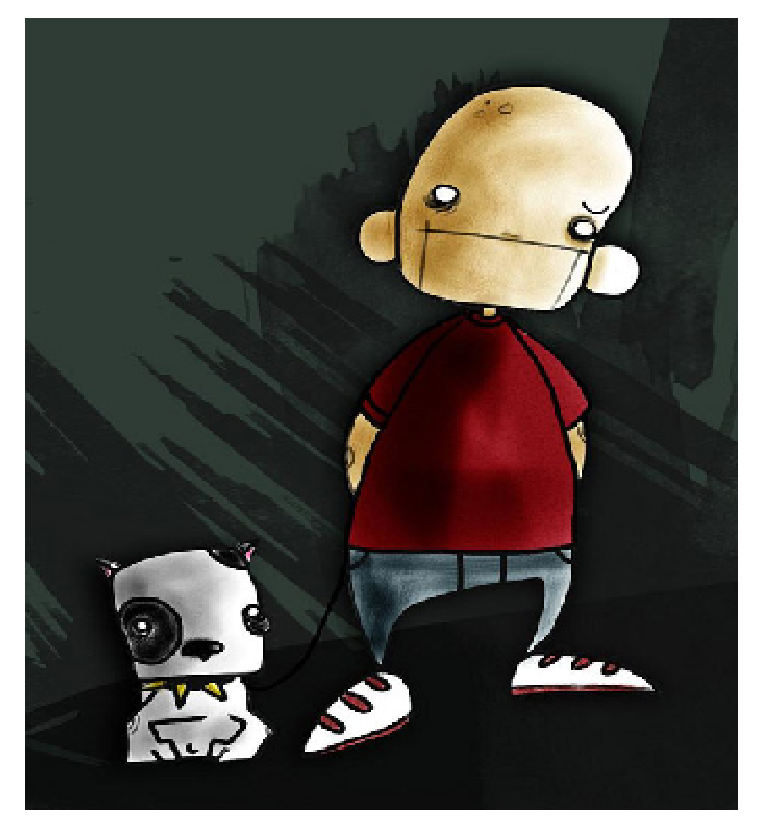
\includegraphics[scale=0.4]{a-fig1}
%\caption{Tobi y su perro}
\end{center}
}
\end{minipage}

\section*{¿Qué pasó con Tobi?}
\begin{itemize}
\item Es posible que el pequeño profesor no haya aplicado la metodología adecuada
\item Otra hipótesis es que Tobi no posea la capacidad para aprender a silbar
\item Una tercera hipótesis, es que a Tobi no le interesa aprender a silbar
\end{itemize}

\section*{Análisis de este caso}
\begin{itemize}
\item El interés y la necesidad de aprender algo, tienen que nacer de adentro
\item La función del profesor, es estimular que se genere esa necesidad y facilitar que esa necesidad pueda satisfacerse 
\end{itemize}

\section*{Conclusiones}
\begin{itemize}
\item Nadie puede aprender por otros, el interés por el aprendizaje debe generarse en el interior de la persona
\item Las materias no tiene una existencia real aunque estén escritas en los libros, lo que existe son las personas y sus problemas, por tanto es menos importante almacenar información y es mas importante el interés por aprender
\item Las personas aprenden lo que les interesa
\end{itemize}
\newpage{\pagestyle{empty}\cleardoublepage}
%%\newpage{\pagestyle{empty}\cleardoublepage}
\tableofcontents %\mainmatter \listoftables \listoffigures
%\mainmatter %comienza a enumerar desde aqui
%\chapter*{Introducci�n\markboth{Introducci�n}{Introducci�n}}
%\label{sec:introduccion}
%\addcontentsline{toc}{chapter}{Introducci�n}%para que no lo enumere
%%++++++++++++++++++++++++++++++++++++++++++++++++++++++++++
\mainmatter
\chapter{Introducci�n}
%%%BEGIN+++++++++ induccionEM.tex +++++++++++++++++

El principio de inducción fue formulado por Michael Faraday  (Inglaterra) e independientemente por Joseph Henry (Estados Unidos) en el a\~no de 1831~\cite{}. Hoy en día, este principio es la base para producir la electricidad en la centrales hidroeléctricas que posteriormente es conducida hasta nuestros hogares.

\section{Flujo magnético}

\begin{figure}[h]
\begin{center}
\includegraphics[scale=0.8]{induccionEM/flujoB-definicion.pdf}
\end{center}
\caption{Flujo magnético atravezando la superficie $A$.}
\label{fig:flujoB-def}
\end{figure}
%
Se define el flujo agnético $\Phi_B$ a través de la superficie de área $A$ como
\begin{align}
\Phi_B=\int_A \vec{B}\cdot d\vec{A}\,,
\end{align}
donde $d\vec{A}$ es un vector normal a la superficie, y forma un ángulo $\theta$ con el vector $\vec{B}$, tal como se muesstra en la Fig.~\ref{fig:flujoB-def}. La integral debe realizarse sobre toda el área $A$. 

\section{Principio de inducción}

%%%END+++++++++ induccionEM ++++++++++++++++++++++
\chapter{Gravitaci�n}
%%%%%%%%%%%%%%%%%%%% BEGIN GRAV %%%%%%%%%%%%%%%%%
\section{Movimiento planetario}

Uno de los problemas fundamentales del pensamiento del hombre en la antigüedad, fue el movimiento de los cuerpos celestes. Este pensamiento impulsó el desarrollo de la ciencia hasta nuestros días. Inicialmente para explicar el movimiento de las estrellas errantes y de las estrellas fijas en el cielo, se desarrollaron los siguientes modelos planetarios. 

\subsection{Modelos planetarios}

\begin{enumerate}
\item \textbf{Modelo geocéntrico:} Este primer modelo fue formulado en el año $100$ por el astrónomo griego Ptolomeo de Alejandría. En este sistema la tierra era el centro del universo y el conjunto de las estrellas fijas inundaban el universo circundante alrededor de la tierra. Por otro lado, se asumió que las estrellas errantes que se observaban en la noches giraban en torno a la tierra, algunas describiendo trayectorias muy complicadas, conocidas como epiciclos~\cite{alonso-z}. Cabe anotar que este modelo tenía como fundamentación al ``hombre como el centro del universo'', fue apoyado fuertemene por la iglesia y prevaleció por alrededor de 1400 años.

\item \textbf{Modelo heliocéntrico:} Este modelo fue propuesto por el astrónomo polaco Nicolás Copérnico ($1473-1543$). Tiene como fundamentación al sol como el centro del universo.
Cabe anotar que la idea de tener al sol como centro del universo, no era una idea nueva. Se tienen datos históricos que argumentan que fue realmente una idea del filósofo Aristarco de Samos, muchos años atrás~\cite{alonso-z}.
\end{enumerate}

Cabe mencionar que los dos modelos anteriores lograron explicar el movieminto de las estrellas de una manera aceptable. Sin embargo, prevalecian algunos detalles que necesitaron un estudio y una compresion más profunda de los mismos. Pasados unos años, el físico Johanes Kepler ($1571-1630$) usó el modelo de Copérnico y descubrió las leyes planetarias después de hacer un cuidadoso análisis de los datos coleccionados por el astrónomo danes Tycho Brahe ($1546-1601$). Éste último murió sin poder dar una buena interpretación de sus datos, coleccionados durante toda su vida.
No obstante, estas leyes fueron empíricas y su explicación teórica fue dada unos años después por el Físico británico Isacc Newton ($1642-1727$). Este último hizo la contribución más notable a la dinámica de los cuerpos celestes, que hoy en día conocemos como la ley de la gravitación universal, formulada en el año $1686$ y publicada en el año de $1687$ en el famoso libro; ``Los Principia" (Philosophiae Naturalis Mathematica~\cite{Whitehead:268025}).



%%%%%%%%%%%%%%%%%%%%%%%%%%%%%%%%%%%%%%%%%%%%%%%%%%%%%%%
\subsection{Leyes de Kepler}

\begin{enumerate}
\item \textbf{LEY $1$}: Todos los planetas se mueven en órbitas elípticas con el sol en una de sus focos (ver Fig.~\ref{fig:ley1}).
%%%%%%%%%%%%%%%%
\begin{figure}[h]
\begin{center}
\includegraphics[scale=0.4]{gravitacion/g-ley1}
\end{center}
\caption{Primera ley de Kepler.}
\label{fig:ley1}
\end{figure}
%%%%%%%%%%%%%%%

Dicha ley generó una gran controversia para la época, debido a que las órbitas propuestas por el modelo heliocéntrico de Copérnico eran circulares y reflejaban la perfección del cielo. Las órbitas elípticas habían obstaculizado el trabajo Tycho Brahe durante toda su vida.
Cabe anotar que esta ley fue empírica. Fue deducida de la observación astronómica. Sin embargo, es un resultado de las estructura funcional de la fuerza de gravitación universal, la cual estudiaremos posteriormente.

\item \textbf{LEY $2$}: El radio-vector dirigido desde el sol a un planeta, barre áreas iguales en tiempos iguales (ver Fig.~\ref{fig:ley2}).
%%%%%%%%%%%%%%%%%
\begin{figure}[h]
\begin{center}
\includegraphics[scale=0.4]{gravitacion/g-ley2}
\end{center}
\caption{Segunda ley de Kepler.}
\label{fig:ley2}
\end{figure}
%%%%%%%%%%%%%%%%

Kepler obtuvo dicha ley estudiando detenidamente los datos obtenido en las observaciones astronómicas de Tycho Brahe. En la Fig.~\ref{fig:ley2} podemos ver que el área barrida en un tiempo $t$ fijo, siempre es $A$. 

Veamos las primeras implicaciones de esta ley. Supongamos que un planeta de masa $m$ está en órbita elíptica alrededor del sol. Consideremos un diferencial de área $dA$, tal como se muestra en la Fig.~\ref{fig:dA}.
%%%%%%%%%%%%%%%%%
\begin{figure}[h]
\begin{center}
\includegraphics[scale=0.7]{gravitacion/g-dA}
\end{center}
\caption{Diferencial de área.}
\label{fig:dA}
\end{figure}
%%%%%%%%%%%%%%%%
\begin{equation}
dA = \dfrac{|\vec{r} \times d\vec{r}|}{2} 
\Rightarrow \dfrac{dA}{dt} = \dfrac{1}{2m}|\vec{r} \times m \dfrac{d\vec{r}}{dt}| = \dfrac{1}{2m}|\vec{r}\times \vec{p}|=\dfrac{|\vec{L}|}{2m}\,,
\label{ec:dA}
\end{equation}
donde $\vec{p}$ y $\vec{L}$ son el momento lineal y angular de la masa.
Así, de la ec.~\ref{ec:dA} queda claro que el hecho de que se barran áreas iguales en tiempos iguales tiene como consecuencia que el momento angular $\vec{L}$ de los planetas alrededor del sol es constante, es decir:
\begin{equation}
\vec{L}=\vec{r}\times \vec{p}=\vec{cte}\,.
\end{equation}
Además, esto establece uno de los precedentes fundamentales para la formulación de la ley de la gravitación universal. El hecho de que el momento angular sea una constante implica que la fuerza que está actuando sobre los planetas, es una fuerza central. Esto puede verse de la siguiente forma:
\begin{equation}
\vec{L}=\vec{r} \times \vec{p} \Rightarrow \dfrac{d\vec{L}}{dt}=\dfrac{d}{dt}(\vec{r}\times \vec{p}) =\dfrac{d\vec{r}}{dt}\times \vec{p} + \vec{r} \times \dfrac{d\vec{p}}{dt} = \vec{r} \times \dfrac{d\vec{p}}{dt}\,.
\label{ec:L-constante}
\end{equation}
Por lo tanto, el torque neto $\vec{\tau}$ que actúa sobre cada planeta, debido a su interacción con el sol, está dado por:
\begin{equation}
\vec{\tau}= \dfrac{d\vec{L}}{dt}= \vec{r}\times \dfrac{d\vec{p}}{dt} = \vec{r} \times \vec{F}\,,
\end{equation}
donde $\vec{F}$ es la fuerza neta que actúa sobre cada planeta. Ahora, si $\vec{L}$ es una constante, entonces la ecuación anterior implica que $\vec{r}\times \vec{F}= \vec{0}$, y por lo tanto $\vec{F}$ y $\vec{r}$ son antiparalelas (fuerza atractiva), es decir, \textit{la fuerza que mantiene en órbita a los planetas alrededor del sol, es una fuerza central atractiva}.\footnote{La fuerza $\vec{F}$ y el vector posición $\vec{r}$ no puden ser paralelos dado que la trayectoria es una curva cerrada.}

De lo anterior, tenemos que si consideramos dos puntos $p_1$ y $p_2$ sobre la trayectoria elíptica de cada planeta, se cumple que:
\begin{equation}
\vec{L}=\vec{cte} \Rightarrow |\vec{r}_1 \times \vec{p}_1 |=|\vec{r}_2 \times \vec{p}_2 | \Rightarrow |\vec{r}_1 \times m\vec{v}_1 |=|\vec{r}_2 \times m\vec{v}_2 |\,. \nonumber
\end{equation}
\begin{equation}
\Rightarrow|\vec{r}_1 \times \vec{v}_1 |=|\vec{r}_2 \times \vec{v}_2 |.
\end{equation}
%%%%%%%%%%%%%%%%%
\begin{figure}[h]
\begin{center}
\includegraphics[scale=0.8]{gravitacion/g-perihelio}
\end{center}
\caption{Perihelio y afelio de los planetas.}
\label{fig:relacion-vr}
\end{figure}
%%%%%%%%%%%%%%%%
En el caso particular del perihelio y el afelio  mostrado en la Fig.~\ref{fig:relacion-vr}:
\begin{equation}
|\vec{r}_1 \times \vec{v}_1 |=|\vec{r}_2 \times \vec{v}_2 |\Rightarrow v_1r_1 =v_2r_2 \Rightarrow 
\boxed{\dfrac{v_1}{v_2}=\dfrac{r_2}{r_1}}\,.
\end{equation}
De la ecuación anterior se puede inferir claramente que la rapidez de los planetas al pasar cerca al punto más cercano al sol, debe ser mayor a la rapidez que tengan dichos planetas cuando pasan por el punto más alejado del sol, es decir, la rapidez en el perihelio es mayor a la rapidez en el afelio.

\item \textbf{LEY $3$:} El cuadrado del periodo orbital $P$ de cualquier planeta es proporcional al cubo del semieje mayor $a$ de la órbita elíptica.

De acuerdo a la Fig.~\ref{fig:relacion-vr}:

\begin{equation}
P^2= k a^3 ,
\end{equation}

donde $k$ es una constante a determinar.

\end{enumerate}











%%%%%%%%%%%%%%%%%%%%%%%%%%%%%%%%%%%%%%%%%%%%%%%%%%%%%%%%%%%%%%%%%%
\section{Ley de Gravitación Universal}

En $1688$ Isaac Newton logró establecer con ayuda de las leyes de Kepler, la ley que gobierna el movimiento celeste de los cuerpos. Newton determinó que \textbf{cada partícula del universo atrae a los demás partículas del universo con una fuerza que es directamente proporcional al producto de sus masas e inversamente proporcional al cuadrado de la separación entre dichas masas}.

\begin{figure}[h]
\begin{center}
\includegraphics[scale=0.9]{gravitacion/fuerzagravitacional}
\end{center}
\label{fuerzagravitacional}
\caption{Fuerza de interacción gravitacional}
\end{figure}

Supongamos que tenemos dos partículas ``puntuales'' cuya separación es $r$, entonces, la fuerza que siente la partícula de masa $m_1$ debido a la partícula de masa $m_2$ es:

\begin{equation}
\boxed{
\vec{F}_{12}= G \dfrac{m_1m_2}{r^2}\hat{u}_r = -\vec{F}_{21}
} 
\end{equation}

donde $G$ es conocida como la constante gravitacional; $G=6.673 \times 10^{-11}$ Nm$^2$/kg$^2$. Note que $\vec{F}_{12}$ y $\vec{F}_{21}$ forman un \textbf{par acción-reacción} y además son fuerzas atractivas.



\subsection{Ejemplos:}

\begin{enumerate}

%ejercicio1
\item Ley de kepler para un MCU





%%%%%%%%%%%%%%%%%%%%%%%%% EJEMPLO 2 %%%%%%%%%%%%%%%%%%%%%%%%%%%%%%%%%%%
\vspace{0.5 cm}
%ejercicio2
\item Dos estrellas de masas $m$ y $M$ separadas por una distancia $d$, giran en  órbita circular alrededor de su centro de masa CM, tal como se muestra en la parte izquierda de la Fig.~\ref{fig:sistema-binario-Mm}. 
%
\begin{figure}[h]
\begin{center}
\includegraphics[scale=0.6]{gravitacion/sistema-binario-Mm}\hspace{1.0 cm}
\includegraphics[scale=0.6]{gravitacion/sistema-binario-mm}
\end{center}
\caption{Sistema binario de estrellas en órbitas circulares con distintas e iguales masa.}
\label{fig:sistema-binario-Mm}
\end{figure}
%
\begin{enumerate}
\item Determinar el periodo de cada estrella.
\item Suponga que $M\gg m$. En este caso, se puede asumir que la masa $M$ está en el centro de masa del sistema. 
¿Cuál es el periodo en este caso? ¿Es compatible con la tercera Ley de Kepler para el movimiento elíptico con excentricidad 0 (órbita circular)?
%
\item El sistema binario Plaskett consiste de dos estrellas de masas iguales girando en torno a su centro de masa CM, tal como se muestra en la parte derecha de la Fig.~\ref{fig:sistema-binario-Mm}. 
La rapidez de cada estrella es aproximadamente $v = 300$ km/s y el periodo orbital es de $14,396$ días~\url{https://en.wikipedia.org/wiki/Plaskett%27s_Star}. 
Use el resultado del primer literal para determinar la masa $m$ de cada estrella.
\end{enumerate}

Solución:
\begin{enumerate}

\item En primer lugar,  sabemos que la fuerza que experimenta la masa $M$ debido a su interacción con la masa $m$ esta dada por ley de gravitación universal:
%
\begin{align}
\label{ec1:LGU-eje2}
F=\,&G \dfrac{Mm}{d^2}
\end{align}

Por otro lado, sabemos que la fuerza gravitacional que actúa sobre las masas es de carácter central y que el movimiento alrededor de su centro de masa es circular uniforme con distintos radios $r_1$ y $r_2$, pero con igual velocidad angular $\omega$. 
Por lo tanto, la fuerza que experimenta la masa $M$ debido a su interacción con la masa $m$ está dada por:
%
\begin{align}
\label{ec2:LGU-eje2}
F=\,& M\dfrac{v_2^2}{r_2}=M\omega^2r_2\,.
\end{align}
%
Note que usamos la relación $v=\omega r$, para un movimiento circular uniforme. 

Análogamente, la fuerza central que experimenta la masa $m$ debido a su interacción con la masa $M$ está dada por la siguiente expresión:
%
\begin{align}
\label{ec3:LGU-eje2}
F=\,& m\dfrac{v_1^2}{r_1}=m\omega^2r_1\,.
\end{align}
%
Ahora, si multiplicamos la ec.~\eqref{ec2:LGU-eje2} la masa $m$ y la ec.~\eqref{ec3:LGU-eje2} la masa $M$ y las sumamos, tenemos la siguiente ecuación:
%
\begin{align}
\label{ec4:LGU-eje2}
F(m + M) =\,& \omega^2Mm\left(r_1+r_2\right)\,.
\end{align}
%
Despejando la fuerza $F$ de la ec.~\eqref{ec1:LGU-eje2} y reemplazando en la ec.~\eqref{ec4:LGU-eje2}, tenemos que:
%
\begin{align}
\label{ec5:LGU-eje2}
G\dfrac{Mm}{d^2}(m+M)=\,&\omega^2Mm\left(r_1+r_2\right)\,.
\end{align}
%
Finalmente, usamos la definición del periodo en un movimiento circular uniforme $P=\dfrac{2\pi}{\omega}$ y la relación $r_1+r_2=d$ mostrada en la Fig.~\ref{fig:sistema-binario-Mm}, para concluir que:
%
\begin{align}
\label{ec6:LGU-eje2}
P^2=\,&\dfrac{4\pi^2}{G(m+M)}d^3\,.
\end{align}

\item Si asumimos que $M\gg m$ en la ec.~\eqref{ec5:LGU-eje2}, entonces:
%
\begin{align}
\label{ec7:LGU-eje2}
P^2~\approx\,&\dfrac{4\pi^2}{GM}d^3\,,
\end{align}
es decir, obtenemos la tercera ley de Kepler para el caso de un movimiento circular. Recordemos que esta ley fue originalmente deducida para el sistema planetario en el cual la masa del sol es mucho mayor que la masa de los planetas, y en este contexto la aproximación $M\gg m$ es completamente válida. De igual forma, es importante aclarar, que las órbitas planetarias realmente son elípticas en las cuales la distancia $d$ debe ser interpretada como el semieje mayor de la elipse (parámetro comúnmente llamado $a$). Por lo tanto, podemos afirmar que este resultado es compatible con la tercera ley de Kepler.

\item Usando la ec.~\eqref{ec6:LGU-eje2} con $M=m$, tenemos que:
%
\begin{align}
\label{ec8:LGU-eje2}
m=\,&\dfrac{2\pi^2 d^3}{G P^2}\,,
\end{align}
%
además, en el movimiento circular se cumple que:
\begin{align}
\label{ec9:LGU-eje2}
P=\,&\dfrac{2\pi}{\omega}=\dfrac{2\pi R }{v}=\dfrac{\pi d}{v}\,,
\end{align}
donde usamos la relación $R=d/2$ entre el diámetro y el radio de la órbita circular.
Combinando las dos últimas ecuaciones tenemos que:
\begin{align}
m=\,&\dfrac{2v^3P}{\pi G} = \dfrac{2\times(3\times 10^5\, \text{m/s})^3\times ( 14.396 \times 24\times 3600\, \text{s})}{\pi\times 6,673\times 10^{-11} \text{Nm}^2/\text{kg}^2}
\approx 3.204\times 10 ^{32}\, \text{kg}\,,
\end{align}
%
es decir, alrededor de cien veces la masa del sol ($M_{\odot}\approx 1.988 \times 10^{30}\,\text{kg}$).
\end{enumerate} 





\vspace{0.5 cm}
%%%%%%%%%%%%%%%%%%%%%%%%% EJEMPLO 3 %%%%%%%%%%%%%%%%%%%%%%%%%%%%%%%%%%%
\item Suponga que un satélite de masa $m=2000$ kg está en órbita elíptica alrededor de la tierra.
En el perigeo (punto de mayor cercanía a la tierra) tiene una altitud de 1100 km y en el apogeo (punto de mayor lejanía a la tierra) tiene una altura de 4100 km. 
Suponga que se quiere transferir el satélite desde la órbita elíptica a la órbita circular 
cambiando su velocidad en el perigeo, tal como se muestra en la Fig.~\ref{fig:cambio-orbita}. 
Asuma que el radio terrestre es $R\approx 6400$ km. 
%
\begin{figure}[h]
\begin{center}
\includegraphics[scale=0.8]{gravitacion/cambio-de-orbita}
\end{center}
\caption{Cambio de órbita de un satélite.}
\label{fig:cambio-orbita}
\end{figure}
%
\begin{enumerate}
\item Determinar la energía mecánica del satélite en ambas órbitas.
\item Determinar la excentricidad de la órbita elíptica.
\item ¿Cuál debe ser el cambio en la velocidad del satélite en el perigeo para realizar la transferencia hacia la órbita circular?
\item Determinar el momento angular en ambas órbitas.
\end{enumerate}

Solución:
\begin{enumerate}
\item La energía mecánica de un cuerpo de masa $m$ en un órbita elíptica alrededor de un cuerpo de masa $M\gg m$ esta dada por la expresión:
%
\begin{align}
\label{ec1:eje3}
E=\,&-\dfrac{GmM}{2 a}\,,
\end{align}
%
donde $a$ es el semieje mayor de la órbita. 
Por lo tanto, la energía mecánica en la órbita elíptica es: 
%
\begin{align}
\label{ec2:eje3}
E_1=\;&-\dfrac{GmM}{2 a} = -\left(\dfrac{GM}{R^2}\right)\dfrac{mR^2}{2a}=-g\dfrac{mR^2}{2a}
\end{align}
%
donde $g=9.8\; \text{m}/\text{s}^2$ es la aceleración de la gravedad sobre la superficie terrestre. Reemplazando los valores numéricos:
%
\begin{align}
\label{ec3:eje3}
E_1=\;& -9.8\; \text{m}/\text{s}^2 \left(\dfrac{2\times 10^3 \text{kg}\times (6400\times 10^3 \text{m})^2}{\left(1100+4100+2(6400)\right)\times 10^3 \text{m}}\right)\approx -4.46 \times 10^{10} \text{J}\,.
\end{align}
%
Análogamente, en la órbita circular, la energía mecánica también está dada por la ec.~\eqref{ec1:eje3}, donde ahora el semieje mayor de la órbita debe ser interpretado como la distancia que hay al perigeo, es decir:
%
\begin{align}
\label{ec4:eje3}
E_2=\;& -9.8\; \text{m}/\text{s}^2 \left(\dfrac{2\times 10^3 \text{kg}\times (6400\times 10^3 \text{m})^2}{2\left(1100+6400\right)\times 10^3 \text{m}}\right)\approx -5.35 \times 10^{10} \text{J}\,.
\end{align}

\item La excentricidad de la órbita elíptica puede determinarse usando la expresión:
\begin{align}
\label{ec5:eje3}
\epsilon=\;& \dfrac{r_{\text{max}}-r_{\text{min}}}{r_{\text{max}}+r_{\text{min}}}\,,
\end{align}
%
donde $r_{\text{max}}$ y $r_{\text{min}}$ son respectivamente las distancias al apogeo y al perigeo de la órbita elíptica. Recuerde que estas son las distancias de mayor lejanía y mayor cercanía entre los centros de masa de ambos cuerpos. En este caso:
\begin{align}
\label{ec6:eje3}
\epsilon=\;& \dfrac{((R+4100)-(R+1100))\;\text{km}}{((R+4100)+(R+1100))\;\text{km}}=\dfrac{3000}{(2R+5200)}=\dfrac{3000}{12800+5200}=\dfrac{1}{6}\,.
\end{align}

\item Para determinar el cambio en la velocidad del satélite, calculemos primero su rapidez en el perigeo para cada una de las dos órbitas. En este punto esta rapidez es fija una vez se tiene una órbita de movimiento.
Para lo anterior, usaremos la definición de la energía mecánica para la órbita elíptica en el perigeo:
%
\begin{align}
\label{ec7:eje3}
E_1=&\;-G\dfrac{M\,m}{r_{\text{min}}}+\dfrac{1}{2}m\, v_1^2\,,
\end{align}
%
Por lo tanto:
%
\begin{align}
\label{ec8:eje3}
v_1=\sqrt{\dfrac{2}{m}\left(E_1+G\dfrac{m\,M}{r_{\text{min}}}\right)}
=\sqrt{\dfrac{2}{m}\left((E_1+g\dfrac{mR^2}{r_{\text{min}}}\right)}\,,
\end{align}
donde usamos nuevamente el valor de la gravedad sobre la superficie terrestre.
%
Finalmente, podemos concluir que el cambio en la rapidez está dado por:
\begin{align}
\label{ec9:eje3}
\Delta v =&\; (v_2-v_1)=\sqrt{\dfrac{2}{m}}\left[\sqrt{\left(E_1+g\dfrac{mR^2}{r_{\text{min}}}\right)}-\sqrt{\left(E_2+g\dfrac{mR^2}{r_{\text{min}}}\right)}\right]\approx -584.784\; \text{m/s} \,,
\end{align}
%
donde tuvimos en cuenta que la rapidez $v_2$ tiene la misma estructura de la ec.~\eqref{ec8:eje3} cambiando $E_1$ por la energía $E_2$. De este resultado se puede concluir que el satélite debe disminuir su velocidad para poder pasar desde la órbita elíptica a a la órbita circular.

\item El momento angular en ambas órbitas es respectivamente:
\begin{align}
L_1=&\; |\vec{r}_1\times \vec{p}_1|= m\, r_{\text{min}}v_1 \approx 1.18531\times10^{14}\; \text{kg m}^2/\text{s}\\
L_2=&\;|\vec{r}_2\times \vec{p}_2|= m\, r_{\text{min}}v_2 \approx 1.09759\times10^{14} \; \text{kg m}^2/\text{s}\,.
\end{align}


\end{enumerate}


















\end{enumerate}






\subsection{Ejercicios:}
\begin{enumerate}

\item Suponga que el movimiento de la tierra alrededor del sol es casi circular (la excentricidad $e$ de la órbita de la tierra es casi $0$) y determine la constante $k$ que aparece en la tercera ley del Kepler $P^2=ka^3$.

\item Calcule la masa el sol usando el periodo de rotación de la tierra alrededor del sol $P \approx 356$ días $\approx 3.156 \times 10^7$ s y sabiendo que la distancia tierra sol es $r \approx 1.496 \times 10^{11}$ m (distancia desde el centro de la tierra al centro del sol).

\item Calcule el valor de la gravedad terrestre usando el radio de la tierra $R\approx 6.37 \times 10^6$ m y la masa de la tierra $M \approx 5.98 \times 10^24$ kg.

\item Considere un satélite de masa $m$ que se mueve en órbita circular alrededor de la tierra con una rapidez $v$ constante y a una altura fija $h$ sobre la superficie terrestre. Si el satélite es geoestacionario (permanece en una posición fija sobre la tierra), ¿qué tan rápido debe moverse? y ¿a qué altura?\\
\textit{Respuesta:} $v=3.07 \times 10^3$ m/s, $h \approx 36000$ km.

\item Si el periodo de la luna alrededor de la tierra es de $28$ días, ¿cuál debe ser el periodo de un satélite que órbita la tierra a una distancia $1/10$ de la distancia tierra - luna?\\
\textit{Respuesta:} $T=28$ $(1/10^{3/2})$ días.

\end{enumerate}









%%%%%%%%%%%%%%%%%%%%%%%%%%%%%%%%%%%%%%%%%%%%%%%%%%%%%%%%%%
\section{Campo Gravitacional}

Supongamos que tenemos una masa puntual $m$ y a diferentes posiciones de $m$ ponemos una masa puntual $m'$. En cada posición $m$ experimenta una fuerza $\vec{F}$ debido a la atracción gravitacional.

\begin{figure}[h]
\begin{center}
\includegraphics[scale=0.8]{gravitacion/campo}
\label{campo}
\end{center}
\caption{Campo gravitacional generado por una masa puntual $m$}
\end{figure}

El campo gravitacional en un punto $P$ producido por la masa $m$ es definido como la fuerza ejercida sobre una unidad de masa $m'$ colocada en $P$, es decir, es la fuerza ejercida sobre una masa de prueba $m'$ dividida sobre $m'$, es decir:

\begin{equation}
\boxed{
\vec{g}_p(r)=\dfrac{\vec{F}}{m'}=-G\dfrac{m}{r^2}\hat{u}_r
}
\end{equation}     

Para el caso general de una distribución de masa volumétrica (Fig.~\ref{fig_distribucion_continuo} ), superficial o lineal; el campo gravitacional se calcula con la siguiente expresión:

\begin{equation}
\boxed{\vec{g}_p(r)=-G\int_M \dfrac{dm}{r^2}\hat{u}_r} ,
\label{ecucampogcontinuo}
\end{equation} 

donde la integral debe hacerse sobre todo el cuerpo de masa $M$. Note que que el la ecuación anterior, el vector unitario $\hat{u}_r$ y la magnitud $r$ son variables al igual que $dm$, tal como se muestra en la Fig.~\ref{fig_distribucion_continuo}. 

\begin{figure}[h]
\begin{center}
\includegraphics[scale=0.9]{gravitacion/figcampogcontinuo}
\caption{Campo gravitacional generado por una masa  $M$.}
\label{fig_distribucion_continuo}
\end{center}
\end{figure}







%%%%%%%%%%%%%%%%%%%%%%%%%%%%%%%%%%%%%%%%%%%%%%%%%%%%%%%%%%%%%%%%
\subsection{Energía potencial gravitacional $E_p(r)=U_p(r)$}

\begin{figure}[h]
\begin{center}
\includegraphics[scale=0.9]{gravitacion/energiapotencial}
\caption{Energía potencial}
\label{energia potencial}
\end{center}
\end{figure}

Dado que la fuerza gravitacional $\vec{F}_g$ es una fuerza central y sólo depende de la distancia $r$ entre las dos masas (Fig.~\ref{energia potencial} ), entonces $\vec{F}_g$ es una fuerza conservativa y podemos asociarle una función energía potencial gravitacional $E_p(r)$.

\begin{equation*}
\vec{F}_g(r)= -G\dfrac{mm'}{r^2}\hat{u}_r = -\vec{\nabla}E_p(r) = - \hat{u}_r \dfrac{\partial}{\partial r} E_p(r) 
\end{equation*}
\begin{equation*}
\Rightarrow -G \dfrac{mm'}{r^2}=- \dfrac{\partial}{\partial r} E_p(r) \Rightarrow \int _{\infty} ^{r} \dfrac{Gmm'}{r^2}dr = \int_{0}^{E_p} dE_p
\end{equation*}
\begin{equation}
\Rightarrow \boxed{E_p(r)= -\dfrac{Gmm'}{r}} ,
\label{energiag}
\end{equation}
donde hemos definido $E_p(\infty)=0$, es decir, hemos tomado el cero de energía potencial en el infinito.

Para un sistema de $n$ masas puntuales $m_1, m_2, \cdots, m_n$, la energía potencial del sistema está dada por:

\begin{equation}
E_p=U =\dfrac{1}{2}\sum_{i=1}^n\sum_{j=1\neq i}^n \dfrac{-Gm_im_j}{r_{ij}} = \sum_{j<i=1}^{n} \dfrac{-Gm_im_j}{r_{ij}} ,
\end{equation}

donde $r_{ij}$ es la magnitud del vector posición que va desde la masa $m_i$ hasta la masa $m_j$.\\

\subsection*{Ejemplos}

\begin{itemize}
\item Para dos masas puntuales $m_1$, $m_2$, separadas una distancia $r=r_{12}$:
\begin{equation}
U=-G \dfrac{m_1m_2}{r_{12}}=-G \dfrac{m_1m_2}{r}
\end{equation}
\item Para tres masas puntuales $m_1$, $m_2$, $m_3$, separadas distancias $r_{12}$, $r_{13}$, $r_{23}$ (ver Fig.~\ref{figtresmasas} para mayor ilustración):
\begin{eqnarray}
\nonumber
U&=&-G \dfrac{m_1m_2}{r_{12}}-G \dfrac{m_1m_3}{r_{13}}-G \dfrac{m_2m_3}{r_{23}} \\
&=&-G\bigg(\dfrac{m_1m_2}{r_{12}}+ \dfrac{m_1m_3}{r_{13}}+\dfrac{m_2m_3}{r_{23}})
\end{eqnarray}
\begin{figure}
\begin{center}
\includegraphics[scale=0.9]{gravitacion/tresmasas}
\end{center}
\caption{Tres masas puntuales}
\label{figtresmasas}
\end{figure}
\item Para cuatro masas puntuales $m_1$, $m_2$, $m_3$, $m_4$, separadas distancias $r_{12}$, $r_{13}$, $r_{14}$, $r_{23}$, $r_{24}$, $r_{34}$:
\begin{eqnarray}
\nonumber
U=-G\bigg(\dfrac{m_1m_2}{r_{12}}+ \dfrac{m_1m_3}{r_{13}}+\dfrac{m_1m_4}{r_{14}}+\dfrac{m_2m_3}{r_{23}}+\dfrac{m_2m_4}{r_{24}}+\dfrac{m_3m_4}{r_{34}}\bigg)
\end{eqnarray}
\end{itemize}

\subsection*{Ejemplo}
Un proyectil de masa $m$ es lanzado desde la superficie de la tierra formando un ángulo $\alpha$ con la vertical tal como se muestra en la Fig.~\ref{fig-tiro}. Si la rapidez inicial del proyectil es $v_0=\sqrt{\dfrac{GM}{R_e}}$, donde $M$ es la masa de la tierra, determinemos la altura máxima alcanzada por el proyectil (\textbf{$r_{max}$}).\cite{klepner} \cite{youngfisica}

\begin{figure}[h]
\begin{center}
\includegraphics[scale=0.3]{gravitacion/tiro}
\end{center}
\caption{Altura máxima ($r_{max}$) en un tiro parabólico}
\label{fig-tiro}
\end{figure}

Usando la conservación de la energía mecánica del sistema masa-tierra, tenemos:
\begin{eqnarray}
\dfrac{1}{2}m v_{0}^{2} - \dfrac{GmM}{R}=\dfrac{1}{2}m v^{2} - \dfrac{GmM}{r_{max}},
\end{eqnarray}
donde $v$, es la rapidez cuando se alcanza la altura máxima.

Por otro lado, usando la conservación del momento angular del sistema masa-tierra, tenemos:
\begin{eqnarray}
mRv_{0}\sen{\alpha}=mr_{max}v
\end{eqnarray}
Usando las dos ecuaciones anteriores, tenemos que:
\begin{eqnarray}
r_{max}=R(1+\cos{\theta})
\end{eqnarray}










%%%%%%%%%%%%%%%%%%%%%%%%%%%%%%%%%%%%%%%%%%%%%%%%%%%%%%%%%
\subsection{Potencial gravitacional $V(r)$}

Se define el potencial gravitacional $V(r)$ como la energía potencial por unidad de masa $m'$ colocada en el campo gravitacional.
\begin{equation}
\boxed{V(r)=\dfrac{E_p(r)}{m'}= -\dfrac{Gm}{r}}
\end{equation}

Note que: 
\begin{displaymath}
g(r)=-\dfrac{Gm}{r^2}=-\dfrac{\partial}{\partial r}(-\dfrac{Gm}{r})
\end{displaymath}
\begin{equation}
\Rightarrow \boxed{ \vec{g}(r)= -\vec{\nabla}V(r) }
\label{gradienteg}
\end{equation}

La ecuación anterior es fundamental. El concepto de potencial gravitacional juega un papel muy importante en el cálculo de algunos campos, debido a que es una cantidad escalar, la cual ``casi'' siempre es más fácil de calcular que la cantidad vectorial $\vec{g}$. Una vez calculado $V(r)$ hallamos $\vec{g}$ usando la ec.~\eqref{gradienteg}. 

Definimos la \textbf{superficie equipontencial} como aquella superficie que rodea a la masa $m$ en la cual $V$ tiene el mismo valor.

\begin{figure}[h]
\begin{center}
\includegraphics[scale=0.8]{gravitacion/superficie}
\caption{Superficie equipotenciales de una carga puntual (curva a rayas).}
\label{superficie-equipotencial}
\end{center}
\end{figure}

Para el caso de distribuciones continuas de masa, el potencial gravitacional ha de calculase mediante la ecuación:

\begin{equation}
\boxed{V(r)= -G\int_M \dfrac{dm}{r}}
\end{equation}

\subsubsection{Principio de superposición para masas puntuales}

En cualquier campo $P$ (Fig.~\ref{camposuperposicion} ), el campo debido a un grupo de masas $m_1, m_2, \cdots, m_n$, es igual al vector suma de los campos $\vec{g}_i$ generados por cada una de masas individuales, es decir, el campo en el punto $P$ es la superposición de los campo individuales $\vec{g}_i$:

\begin{figure}[h]
\begin{center}
\includegraphics[scale=0.7]{gravitacion/camposuperposicion}
\end{center}
\caption{Principio de superposición para campos}
\label{camposuperposicion}
\end{figure}

\begin{equation}
\vec{g}=\sum_{i=1}^{n}\vec{g}_i = -\sum_{i=1}^{n}\dfrac{Gm_i}{r_i^2} \hat{u}_i
\end{equation}


Análogamente el potencial en el punto $P$ es:

\begin{equation}
V=\sum_{i=1}^{n}V_i = \sum_{i=1}^{n} \dfrac{-Gm_i}{r_i}
\end{equation}









%%%%%%%%%%%%%%%%%%%%%%%%%%%%%%%%%%%%%%%%%%%%%%%%%%%%%%%%%%%
\section{Movimiento general bajo interacción gravitacional}

Consideremos el movimiento de un cuerpo de masa $m$ alrededor de un cuerpo de masa $M>m$ tal como se muestra en la Fig.~\ref{fig:movimiento-general}.
%%%%%%%%%%%%%%
\begin{figure}
\begin{center}
\includegraphics[scale=1]{gravitacion/g-movimiento-general}
\end{center}
\caption{Movimiento general de un cuerpo bajo interacción gravitacional.}
\label{fig:movimiento-general}
\end{figure}
%%%%%%%%%%%%
Según la conservación de la energía mecánica
\begin{align}
\label{eq:E-mecanica}
E =& \dfrac{1}{2}mv^2 + U(r) = \dfrac{1}{2}m(v_r^2+v_\theta^2) -\dfrac{G m}{r} = \dfrac{1}{2}m\left[\left(\dfrac{dr}{dt}\right)^2+\left(r\dfrac{d\theta}{dt}\right)^2\right] -\dfrac{G m}{r} \nonumber \\
=& \dfrac{1}{2}m\left(\dfrac{d\theta}{dt}\right)^2 \left[\left(\dfrac{dr}{d\theta}\right)^2+r^2\right]-\dfrac{G m}{r}\,.
\end{align}
%
Por otro lado, usando la definición de momento angular
\begin{align}
\label{eq:L}
\vec{L}=m\,\vec{r}\times\vec{v}=m\,\vec{r}\times(\vec{v_r}+\vec{v_\theta})= m\,\vec{r}\times\vec{v_\theta} \to L = m\,r \left(r\dfrac{d\theta}{dt}\right)\,.
\end{align}
Reemplazando la ec.~\eqref{eq:L} en la ec.~\eqref{eq:E-mecanica} tenemos que:
\begin{align}
\label{eq:drdthetat}
\left(\dfrac{dr}{d\theta}\right)^2 = \dfrac{m^2r^4}{L^2}\left(\dfrac{2E}{m}+\dfrac{2GM}{r}-\dfrac{L^2}{m^2r^2}\right)\,.
\end{align}

Por otro lado, en el estudio de la geometría se tiene que la ecuación de las cónicas es
\begin{equation}
\label{eq:conicas}
\dfrac{\epsilon d}{r} = 1 +\epsilon\cos\theta\,,
\end{equation}
donde $\epsilon$ es la excentricidad de la cónica, $d$ es la distancia a la directriz y $r,\theta$ son la coordenadas polares~\cite{alonso1967fundamental}.
Usando esta ecuación se tiene que
\begin{equation}
\label{eq:conica-drdtheta}
\left(\dfrac{dr}{d\theta}\right)^2=\dfrac{r^4\sin\theta^2}{d^2}\,.
\end{equation}
Por lo tanto, de acuerdo a las ecs.~\eqref{eq:drdthetat} y~\eqref{eq:conica-drdtheta} tenemos que:
\begin{align}
\sin\theta^2 =& \dfrac{d^2m^2}{L^2}\left(\dfrac{2E}{m}+\dfrac{2Gm}{r}-\dfrac{L^2}{m^2r^2}\right)=\left(1-\dfrac{d^2}{r^2}+\dfrac{2d}{r\epsilon}-\dfrac{1}{\epsilon^2}\right)\,,
\end{align} 
donde usamos la ec.~\eqref{eq:conicas}. Comparando las potencias en la coordenada $r$ tenemos las siguientes dos relaciones: 
\begin{itemize}
\item Potencias de $r^0$:
\begin{equation}
\label{eq:Energia-general}
1-\dfrac{1}{\epsilon^2}=\dfrac{2d^2mE}{L^2} \to E=\dfrac{L^2}{2d^2m}\left(1-\dfrac{1}{\epsilon^2}\right)\,.
\end{equation}
\item Potencias de $r^{-1}$:
\begin{equation}
\label{e:excentricidad}
\dfrac{2d}{r\epsilon}=\dfrac{2d^2m^2GM}{rL^2} \to \epsilon=\dfrac{L^2}{dm^2GM}\,.
\end{equation}
\end{itemize}

A continuación, en la Tabla~\ref{tab:conicas-interpretacion}. mostramos algunas características de las tres cónicas mostradas, enfatizando en el caso particular de la elipse. 
%%%%%%%%%%%%%
\begin{table}[h]
\begin{center}
\begin{tabular}{|c|c|c|c|}
\hline
Cónica & Excentricidad & Energía & Momento angular \\
\hline
&&&\\
Elipse & $0\leq\epsilon<1$ & $E=-\dfrac{GMm}{2a} < 0$& $L^2=Gm^2Ma(1-\epsilon^2)$\\
&&&\\
\hline
&&&\\ 
Parábola & $\epsilon=1$ & $E= 0$& $L>0$\\
&&&\\
\hline
&&&\\ 
Hipérbola & $\epsilon>1$ & $E> 0$& $L>0$\\
&&&\\
\hline
\end{tabular}
\end{center}
\caption{Energía y momento angular en una órbita elíptica. Recuerde que $\epsilon=0$ es la circunferencia.}
\label{tab:conicas-interpretacion}
\end{table} 
%%%%%%%%%%%
Note que aunque el tamaño de una órbita elíptica está determinado por la energía, es decir $E\approx -1 /a$, la forma de la elipse (excentricidad) está determinado por el momento angular. En general, se pueden tener muchas órbitas elípticas con la misma energía, pero con distinto momento angular. 
%Por ejemplo como se muestra en la Fig.~\ref{fig:}.
 
 
 
 
 
 
 
 
 
 
 
 
 
 
 
 
\section{Distribuciones continuas de masa}


\subsection{Ejemplos de campo gravitacional}

\subsubsection{Campo de una barra}

\begin{enumerate}

\item Una barra delgada de longitud $l$ tiene una masa $m$ uniformemente distribuida tal como muestra en la Fig.~\ref{fig:gravitacion-barra1}. El campo en el punto $P$ a una distancia $d$ por el eje de la barra está dado por:
\begin{figure}[h]
\begin{center}
\includegraphics[scale=0.8]{gravitacion/barra1}
\end{center}
\caption{Campo en el eje de una barra de longitud $l$.}
\label{fig:gravitacion-barra1}
\end{figure}

\begin{eqnarray}
\vec{g}=-G\int_m \dfrac{dm}{r^2}\hat{u}_r = -G\int_m \dfrac{dm}{x^2}(-\hat{i})\,.
\end{eqnarray}
Usando la función densidad lineal de masa:
\begin{displaymath}
\lambda=\dfrac{dm}{dx}=\dfrac{m}{l} \Rightarrow dm=\dfrac{m}{l}dx\,, 
\end{displaymath}
tenemos que:
\begin{equation}
\vec{g}= -G\int_d^{d+l} \dfrac{dm}{x^2}(-\hat{i})=G \dfrac{M}{d(d+l)}\hat{i}\,.
\end{equation}

\item Una barra delgada de longitud $l$ tiene una masa $m$ uniformemente distribuida tal como se muestra en la Fig.~\ref{fig:gravitacion-barra2}. El campo en el punto $P$ está dado por:
\begin{figure}[h]
\begin{center}
\includegraphics[scale=0.9]{gravitacion/barra2}
\end{center}
\caption{Campo en el eje perpendicular a un extremo de una barra de longitud $l$.}
\label{fig:gravitacion-barra2}
\end{figure}
\begin{eqnarray}
\nonumber \vec{g} & = & -G\int_m \dfrac{dm}{r^2}\hat{u}_r =-G\int_m \dfrac{dm}{r^2} (-\cos\theta \hat{i} + \sin\theta \hat{j})  \\ \nonumber
& = &-G\int_m \dfrac{dm}{r^2} (-\dfrac{x}{r} \hat{i} + \dfrac{y}{r} \hat{j}) 
=-G\int_0^l (m/l)dx(-\dfrac{x}{r^3} \hat{i} + \dfrac{y}{r^3} \hat{j}) \\\nonumber
&= &-\dfrac{Gm}{l}\int_0^l dx\Big(-\dfrac{x}{(y^2+x^2)^{3/2}} \hat{i} + \dfrac{y}{(y^2+x^2)^{3/2}} \hat{j}\Big) \\
&=& \dfrac{Gm}{l}\Big(\dfrac{1}{y}-\dfrac{1}{\sqrt{l^2+y^2}}\Big)\hat{i} -\dfrac{Gm}{y}\dfrac{1}{\sqrt{l^2+y^2}}\hat{j}\,.
\end{eqnarray}

\item Caso general: Campo en el punto $P$ mostrado en la Fig.~\ref{fig:gravitacion-barra3}.
\begin{figure}[h]
\begin{center}
\includegraphics[scale=1.2]{gravitacion/barra3}
\end{center}
\caption{Campo general a una distancia $y$ perpendicular al eje de una barra de longitud $l$.}
\label{fig:gravitacion-barra3}
\end{figure}
%
\begin{eqnarray}
\nonumber
\vec{g}&=&-G\int_m \dfrac{dm}{r^2}\hat{u}_r =-G\int_m \dfrac{dm}{r^2} (-\cos\theta \hat{i}+\sin\theta\hat{j}) = -G \lambda \int_m dx \bigg[\dfrac{-x}{r^3}\hat{i}+ \dfrac{y}{r^3}\hat{j}\bigg]\\ \nonumber
&=&-G \lambda \bigg[-\int_{-x_1}^{x_2}\dfrac{x dx}{(x^2+y^2)^{3/2}} \hat{i}+\int_{-x_1}^{x_2}\dfrac{ydx}{(x^2+y^2)^{3/2}}\hat{j}  \bigg] \\ 
&=&-G \lambda \Bigg[\bigg(\dfrac{1}{\sqrt{x_2^2+y^2} }-\dfrac{1}{\sqrt{x_1^2+y^2} } \bigg)\hat{i} + \dfrac{1}{y} \bigg(\dfrac{x_2}{\sqrt{x_2^2+y^2} }+\dfrac{x_1}{\sqrt{x_1^2+y^2} } \bigg)\hat{j} \ \Bigg] \,,
\end{eqnarray}
o alternativamente, usando $x_1=y/\tan\theta_1$ y $x_2=-y/\tan\theta_2$:
\begin{eqnarray}
\vec{g}=\dfrac{-G \lambda }{y}\bigg[(\sin\theta_1 -\sin\theta_2)\hat{i}+(\cos\theta_1 -\cos\theta_2)\hat{j}\bigg]\,.
\end{eqnarray}

En el caso de tener una \textit{barra infinita} de densidad $\lambda$ uniforme podemos usar el resultados anterior con $x_2 \rightarrow \infty$ y $x_1 \rightarrow \infty$ ó $\theta_1 \rightarrow 0$ y $\theta_2 \rightarrow \pi$, tal que:
%
\begin{eqnarray}
\vec{g}(y)=\dfrac{-2G\lambda}{y}\hat{j}\,.
\end{eqnarray}

\textbf{Ejercicio:} Use el resultado general para el campo de una barra y verifique los dos casos particulares hechos con anterioridad.

\end{enumerate}



\subsubsection{Campo de una anillo}
Un anillo de radio $R$ tiene una masa $m$ uniformemente distribuida. El campo $\vec{g}$ en un punto $P$ a lo largo del eje del anillo, tal como se muestra en la Fig.~\ref{fig:gravitacion-anillo}.
%
\begin{figure}[h]
\begin{center}
\includegraphics[scale=0.7]{gravitacion/anillo}
\end{center}
\caption{Campo en el eje de un anillo de radio R.}
\label{fig:gravitacion-anillo}
\end{figure}
%
\begin{eqnarray}
\nonumber \vec{g}
&=&-G\int_m \dfrac{dm}{r^2}\hat{u}_r =-G\int_m \dfrac{dm}{r^2}(\sin\theta \hat{k} - \cos\theta \hat{R}  )\\\nonumber
&=&-G\int_m \dfrac{dm}{r^2}[\sin\theta \hat{k} - \cos\theta (\cos\phi\hat{i}-\sin\phi\hat{j}) ] \\\nonumber
&=&-G\int_0^{2\pi} \dfrac{md\phi}{2\pi} \dfrac{1}{r^2}[\sin\theta \hat{k} - \cos\theta (\cos\phi\hat{i}-\sin\phi\hat{j}) ] \\
&=& -G \dfrac{m2\pi}{2\pi r^2}\sin\theta \hat{k}=-G \dfrac{m}{r^2}\left(\dfrac{z}{r}\right)\hat{k}=-Gm \dfrac{z}{(z^2+R^2)^{3/2}}\hat{k}\,.
\label{ec:campo-gravitacional-anillo}
\end{eqnarray}
Note que en el cálculo anterior usamos:
%
\begin{displaymath}
\lambda=\dfrac{m}{l}=\dfrac{m}{2\pi R}=\dfrac{dm}{dl}=\dfrac{dm}{Rd\phi}\Rightarrow dm=\dfrac{md\phi}{2\pi}\,.
\end{displaymath}


\subsubsection{Campo de una arandela y de un disco}
Considere un disco hueco de radio exterior $R_2$, radio interior $R_1$ y masa $m$ uniformemente distribuida. El campo gravitacional en el punto $P$ mostrado en la Fig.~\ref{fig:gravitacion-arandela} está dado por:
%
\begin{figure}[h]
\begin{center}
\includegraphics[scale=0.9]{gravitacion/arandela}
\end{center}
\caption{Arandela de radio interno $R_1$ y radio externo $R_2>R_1$.}
\label{fig:gravitacion-arandela}
\end{figure}
%
\begin{align}
\vec{g}=&\int_m G\dfrac{dm}{r^2}\hat{u}_r
= \int_m G\dfrac{\sigma\rho d\rho d\phi}{r^2}(\cos\theta \hat{k}-\sin\theta\hat{\rho})\nonumber\\
=& G\int_m\dfrac{\sigma\rho d\rho d\phi}{r^2}\left(\dfrac{z}{r} \hat{k}-\dfrac{\rho}{r} (\cos\phi \hat{i}+\sin\theta\hat{j})\right)
\nonumber\\
=& G\int_{0}^{2\pi}\int_{R_1}^{R_2}\dfrac{\sigma\rho d\rho d\phi}{(z^2+\rho^2)^{3/2}}\left(z \hat{k}-\rho (\cos\phi \hat{i}+\sin\theta\hat{j})\right)\nonumber\\
=& G\int_{R_1}^{R_2}\dfrac{2\pi\sigma\rho d\rho d\phi}{(z^2+\rho^2)^{3/2}} \hat{k}
=\dfrac{2mG}{(R_2^2-R_1^2)} \Bigg(\dfrac{z}{\sqrt{z^2+R_2^2} } - \dfrac{z}{\sqrt{z^2+R_1^2} }  \Bigg)\hat{k}\,.
\label{ec:campo-gravitacional-arandela}
\end{align}
%
Note que si $R_1 \rightarrow 0$, tenemos el campo de un disco o moneda de radio $R_2$:
%
\begin{equation}
\vec{g}(z)=\dfrac{-2mG}{R_2^2} \Bigg(1 - \dfrac{z}{\sqrt{z^2+R_2^2} }  \Bigg)\hat{k}\,.
\label{ec:campo-gravitacional-disco}
\end{equation}
Además, si $R_1 \rightarrow 0$ y $z >> R_2$ tenemos aproximadamente el campo de masa puntual $m$, lo cual es de esperarse ya que desde muy lejos cualquier configuración de masa ha de verse como una masa puntual, tal que:
%
\begin{equation}
\vec{g} \approx -G\dfrac{m}{z^2}\hat{k}\,.
\end{equation}  


\subsubsection{Campo de un plano}
%
\begin{figure}[h]
\begin{center}
\includegraphics[scale=0.6]{gravitacion/plano}
\end{center}
\caption{Plano infinito con densidad superficial de masa $\sigma$.}
\label{fig:gravitacion-plano}
\end{figure}
%
Para calcular el campo de un plano muy grande (infinito) con densidad de masa $\sigma$ uniforme podemos usar el resultado obtenido para el campo de disco dado por la ec.~\ref{ec:campo-gravitacional-disco}. El campo gravitacional del plano se obtiene haciendo infinito el radio del disco, tal como se muestra en la Fig.~\ref{fig:gravitacion-plano}. Es decir:
\begin{align}
\vec{g}=& \lim_{R\to\infty}\dfrac{-2mG}{R^2} \left(1 - \dfrac{z}{\sqrt{z^2+R^2} }  \right)\hat{k} 
= \lim_{R\to\infty}-2\pi\sigma G \left(1 - \dfrac{z}{\sqrt{z^2+R^2} }  \right)\hat{k}\nonumber\\
=& -2\pi\sigma G\, \hat{k}\,,
\label{ec:campo-gravitacional-plano}
\end{align}
donde usamos la función densidad $\sigma=m/(\pi R^2)$.



\subsubsection{Campo de una superficie esférica}
%
\begin{figure}[h]
\begin{center}
\includegraphics[scale=0.9]{gravitacion/esfera1}
\end{center}
\caption{Cascarón esférico de radio R.}
\label{fig:gravitacion-esfera}
\end{figure}
%
Calculemos el campo para un cascarón esférico de radio $R$ y masa $m$ uniformemente distribuida tal como se muestra en la Fig~\ref{fig:gravitacion-esfera}.

\begin{enumerate}
\item Para $r > R$ (exterior del cascarón esférico). De acuerdo a la Fig.~\ref{fig:gravitacion-esfera}:
\begin{eqnarray}
\vec{g}_p=-G\int_m \dfrac{dm}{\rho^2}\hat{u}_{\rho}\,.
\end{eqnarray}
Dada la simetría del problema, al integrar sólo sobrevive la componente del vector $\hat{u}_{\rho}$ en la dirección de $\hat{u}_r$, tal que:
\begin{eqnarray}
\vec{g}=-G\int_m \dfrac{dm}{\rho^2}\hat{u}_{\rho}==-G\int_m \dfrac{dm}{\rho^2} \cos\beta\, \hat{u}_r\,.
\end{eqnarray}
Además, si la distribución superficial de masa $\sigma$ es uniforme, entonces:
\begin{equation}
\sigma=\dfrac{m}{4\pi R^2}=\dfrac{dm}{dA}=\dfrac{dm}{2\pi R^2\sin\theta d\theta} \Rightarrow dm=\dfrac{1}{2}m\sin\theta d\theta ,
\end{equation}
Por otro lado, usando la ley del coseno en el triángulo de lados $r$, $R$ y $\rho$, tenemos:
%
\begin{equation}
\rho^2 =R^2 + r^2 -2Rr\cos\theta.  \hspace{0.5 cm} \text{Derivando} \Rightarrow \sin\theta d\theta = \dfrac{\rho}{Rr} d\rho\,.
\end{equation}
\begin{equation}
R^2=r^2+\rho^2 -2r\rho \cos\beta \Rightarrow \cos\beta =\dfrac{r^2+\rho^2 -R^2}{2r\rho}\,.
\end{equation}
%
Reemplazando las tres ecuaciones anteriores en la ecuación para el campo tenemos que:
\begin{eqnarray}
\vec{g}(r) &=& -\dfrac{Gm}{4Rr^2}\hat{u}_r \int_{r-R}^{r+R} \bigg(1+ \dfrac{r^2-R^2}{\rho^2}  \bigg)d\rho = -G \dfrac{m}{r^2}\hat{u}_r\,.
\label{ec:campo-gravitacional-cascaron}
\end{eqnarray}

\item Para $r < R$ (interior del cascarón esférico). De acuerdo a la Fig.~\ref{fig:gravitacion-esfera}:
\begin{eqnarray}
\vec{g} &=& -\dfrac{Gm}{4Rr^2}\hat{u}_r \int_{R-r}^{r+R} \bigg(1+ \dfrac{r^2-R^2}{\rho^2}  \bigg)d\rho = \hat{0}\,.
\end{eqnarray}
\end{enumerate}

El resultado obtenido para el campo gravitacional de un cascarón esférico, marca uno de los resultados fundamentales en la teoría de campo gravitacional. 
\begin{itemize}
\item El campo gravitacional en el exterior de un cascarón esférico, es equivalente al campo generado por una masa puntual $m$ situada en el centro de masa de dicho cascarón.
\item El campo gravitacional en el interior es nulo. 
\end{itemize}


\subsubsection{Campo de una esfera maciza con densidad de masa uniforme $\rho$}
%
\begin{figure}[h]
\begin{center}
\includegraphics[scale=0.7]{gravitacion/esfera2}
\end{center}
\caption{Esfera maciza de radio $R$ y masa $m$.}
\label{fig:gravitacion-esfera2}
\end{figure}
%
\begin{enumerate}
\item Para $r > R$ (exterior de la esfera), podemos integrar en cascarones esféricos y usar el resultado obtenido para el campo generado por un cascarón de masa diferencial $dm$ en el punto $P$ (ec.~\eqref{ec:campo-gravitacional-cascaron}).
\begin{eqnarray}
\vec{g}(r)=\int_m d \vec{g} = \int_m \bigg(-G \dfrac{dm}{r^2}\hat{u}_r \bigg)=-G \dfrac{1}{r^2}\hat{u}_r\int_m dm= -G \dfrac{m}{r^2}\hat{u}_r\,,
\label{ec:campo-gravitacional-esfera-exterior}
\end{eqnarray}
donde debe quedar claro que ahora $m$ es la masa neta de la esfera maciza.

\item Para $r < R$ (interior de la esfera) sólo contribuye la masa $m'$ localizada en la esfera de radio $r < R$ tal como se muestra en la Fig.~\ref{fig:gravitacion-esfera2} , tal que:
\begin{eqnarray}
\vec{g}(r)=-G \dfrac{m'}{r^2}\hat{u}_r = -G \bigg(m \dfrac{r^3}{R^3} \bigg)\dfrac{1}{r^2}\hat{u}_r= -Gm \dfrac{r}{R^3}\hat{u}_r\,,
\label{ec:campo-gravitacional-esfera-interior}
\end{eqnarray}

donde tuvimos en cuenta que la densidad de la esfera es uniforme, así:
\begin{displaymath}
\rho=\dfrac{m}{\dfrac{4}{3}\pi R^3 } = \dfrac{m'}{\dfrac{4}{3}\pi r^3 } \Rightarrow m'=m \dfrac{r^3}{R^3}\,.
\end{displaymath}

\end{enumerate}

Al igual que el resultado obtenido para el campo gravitacional de un cascarón esférico. El campo de una esfera maciza marca uno de los resultados fundamentales en la teoría de campos. 
\begin{itemize}
\item El campo gravitacional atractivo en el exterior de una esfera, es equivalente al campo generado por una masa puntual $m$ situada en el centro de masa de la esfera. Note que externamente no importa si la masa $m$ está distribuida en un cascarón esférico o en una esfera maciza.
\item El campo gravitacional en el interior, es el campo generado por la masa localizada en una esfera de radio $r < R$, es decir, el campo es generado por la masa que hay desde el punto interno hasta el centro de masa. 
\end{itemize}






\subsection{Ejemplos de potencial gravitacional}


\subsubsection{Potencial de una barra}
Consideremos la barra mostrada en la Fig.~\ref{fig:gravitacion-barra3} de masa $m$ y longitud $l$. El potencial gravitacional en el punto $P$ es:
\begin{align}
V=&-\int_m G\dfrac{dm}{r} = -\int_m G \dfrac{\lambda dx}{r}
=-G\int_{-x_1}^{x_2}\dfrac{\lambda dx}{\sqrt{y^2+x^2}}\nonumber\\
=& -G\lambda \left[\ln\left(\dfrac{\sqrt{x_2^2+y^2}}{y}+\dfrac{x_2}{y}\right)-\ln\left(\dfrac{\sqrt{x_1^2+y^2}}{y}-\dfrac{x_1}{y}\right)\right]\nonumber\\
=& -G\lambda \ln\left(\dfrac{\sqrt{x_2^2+y^2}+x_2}{\sqrt{x_1^2+y^2}-x_1}\right)\,,
\label{ec:potencial-gravitacinal-barra}
\end{align}
donde $\lambda=m/l=m/(x_1+x_2)$ es la densidad de masa de la barra.

%Para el caso de un alambre muy largo (infinito) hacemos $x_1\to\infty$ and $x_2\to\infty$.



\subsubsection{Potencial de un anillo}

Consideremos el anillo de masa $m$ uniformemente distribuida y radio $R$ mostrado en la Fig.~\ref{fig:gravitacion-anillo}. El potencial gravitacional en el punto $P$ es:

\begin{eqnarray}
V=-G\int_m \dfrac{dm}{r}=-G \dfrac{1}{r}\int_m dm =-G \dfrac{m}{r}=-G \dfrac{m}{\sqrt{z^2+R^2}}\,,
\label{ec:potencial-gravitacinal-anillo}
\end{eqnarray}
donde la distancia $r$ desde el diferencial al punto medida $P$ es constante.
Por otro lado, note que:
\begin{eqnarray}
\vec{g}(z)=-\vec{\nabla}V=-\hat{k}\dfrac{d}{dz}V(z)=-Gm \dfrac{z}{(z^2+R^2)^{3/2}} \hat{k}\,.
\end{eqnarray}
Resultado idéntico al obtenido usando la definición de campo (ver ec.~\ref{ec:campo-gravitacional-anillo}). Tenga en cuenta que para este caso particular, ha sido más fácil calcular el potencial y a partir de él calcular el campo gravitacional. 

\textbf{Ejercicio:} Suponga que una masa $m'$ es colocada en el punto $P$. Calcule la rapidez de $m'$ justo cuando pasa por el centro del anillo. ¿Qué condición matemática debe cumplirse para que $m'$ ejecute un movimiento armónico simple? Determine la frecuencia de oscilación.\\
\textit{Respuesta:} 
\begin{displaymath}
v_0=\sqrt{2Gm( \dfrac{1}{R}-\dfrac{1}{\sqrt{R^2+z^2} } )}
\end{displaymath}
Si $z<<R \Rightarrow \dfrac{d^2z}{dt^2}+ \dfrac{Gm}{R^3} z \approx 0$ y así:
\begin{displaymath}
\omega_0=\sqrt{\dfrac{Gm}{R^3} }\,.
\end{displaymath} 



\subsubsection{Potencial de una arandela y un disco}
Calculemos el potencial gravitacional de la arandela de radio exterior $R_2$ y radio interior $R_1<R_2$ en el punto $P$ mostrado en la Fig.~\ref{fig:gravitacion-arandela}.
\begin{align}
V=& -G\int_m \dfrac{dm}{r} = -G\int_0^{2\pi}\int_{R_1}^{R_2}\dfrac{\sigma \rho d\rho d\phi}{\sqrt{z^2+\rho^2}}\nonumber\\
=& -G\int_{R_1}^{R_2}\dfrac{\sigma 2\pi\rho d\rho }{\sqrt{z^2+\rho^2}}=-2\pi\sigma G\left(\sqrt{R_2^2+z^2} -\sqrt{R_1^2+z^2}\right)
\nonumber\\
=& -\dfrac{2G m}{(R_2^2-R_1^2)} \left(\sqrt{R_2^2+z^2} -\sqrt{R_1^2+z^2}\right)\,.
\label{ec:potencial-gravitacional-arandela}
\end{align}
Note que podemos determinar el campo gravitacional a partir de este potencial de la siguiente manera:
\begin{align}
\vec{g}(z)=&-\vec{\nabla}V(z)=-\hat{k}\dfrac{d}{dz}V(z)\nonumber\\
=&\dfrac{2mG}{(R_2^2-R_1^2)} \Bigg(\dfrac{z}{\sqrt{z^2+R_2^2} } - \dfrac{z}{\sqrt{z^2+R_1^2} }  \Bigg)\hat{k}\,,
\end{align}
expresión que fue calculada directamente con la definición del campo gravitacional (ver ec.~\ref{ec:campo-gravitacional-arandela}).

Para un disco de radio $R$ y masa $m$ usamos la ec.~\ref{ec:potencial-gravitacional-arandela} con $R_1=0$ y $R_2=R$, tal que:
\begin{align}
V=& -\dfrac{2G m}{R^2} \left(\sqrt{R^2+z^2} -z\right)=-2\pi G \sigma \left(\sqrt{R^2+z^2} -z\right)\,.
\label{ec:potencial-gravitacinal-disco}
\end{align}



\subsubsection{Potencial de un plano infinito con densidad superficial de masa $\sigma$ constante}

\begin{equation}
V(z)=\lim_{R\to\infty} V_{\text{disco}} 
=\lim_{R\to\infty} \left[-2\pi G \sigma \left(\sqrt{R^2+z^2} -z\right)\right] = -\infty +2\pi G \sigma z\,,
\end{equation}
dado que el potencial es infinito, realizamos el proceso de renormalización. Éste consiste en tomar la parte finita del potencial. Por lo tanto, el potencial renormalizado de un plano infinito de densidad de masas $\sigma$ es:
\begin{equation}
V(z)=2\pi G \sigma z\,.
\label{ec:potencial-gravitacional-plano}
\end{equation} 
Note que podemos determinar el campo gravitacional a partir de este potencial de la siguiente manera:
\begin{eqnarray}
\vec{g}=-\vec{\nabla}V(z)=-\hat{k}\dfrac{d}{dz}(2\pi G \sigma z)=-2\pi\sigma G \hat{k}\,,
\end{eqnarray}
el cual fue calculado directamente con la definición del campo gravitacional (ver ec.~\ref{ec:campo-gravitacional-plano}).



\subsubsection{Potencial de una superficie esférica de radio R} 

\begin{enumerate}
\item Para el exterior del cascarón esférico ($r \geq R$):

\begin{equation}
V=-G \dfrac{m}{r}  
\end{equation}

\item Para el interior del cascarón esférico ($r \leq R$):

\begin{equation}
V=-G \dfrac{m}{R}=cte.
\end{equation}

\end{enumerate}

\subsubsection{Potencial de una esfera maciza de radio R}

\begin{enumerate}
\item Para el exterior de la esfera ($r \geq R$):

\begin{equation}
V=-G \dfrac{m}{r}  
\end{equation}

\item Para el interior de la esfera ($r \leq R$):

\begin{equation}
V=\dfrac{Gm}{2R^3}(r^2-3R^2)
\end{equation}

\end{enumerate}
%%%%%%%%%%%%%%%%%%%% END GRAV %%%%%%%%%%%%%%%%%%%%%%%%%%%%%%
\chapter{Electrost�tica}
%\documentclass[letterpaper,12pt]{book}
%\usepackage[spanish]{babel}
%\usepackage{graphicx, color}
%\usepackage{amsmath}
%\usepackage{amscd}
%\usepackage{titlesec}
%\usepackage[latin1]{inputenc}
%\usepackage{listings}
%\usepackage{multicol}
%\usepackage{enumerate}
%\usepackage{amssymb}
%\usepackage{amsthm}
%\usepackage{syntonly}
%\usepackage{fancyhdr}
%\usepackage{verbatim}
%\usepackage{fancyvrb}
%\usepackage{hyperref}
%
%\begin{document}

%%%++++++++++++++++++++++++++++++++++++

Claramente los experimentos de frotaci�n pueden electrificar un cuerpo, lo cual se ve claramente en la atracci�n de pedasitos de papel cuando le arrimamos una barra de vidrio o de pl�stico que frotamos previamente. El fen�meno de electrificci�n tambi�n puede verse en las chispas que salen cuando nos quitamos una camisa en ciertos lugares relativamente secos.

\section{Carga el�ctrica}
Experimentalemente \textbf{Benjamin Franklin (1706-1790)} fue quien determin� que existen dos tipos de cargas el�ctricas a las que llam� positivas y negativas. �l determin� que dos barras de vidrio o dos barras de hule (caucho) cargadas por frotaci�n se repelen y dos barras, una de vidrio y otra de hule cargadas, se atraen. El experimento es exquematizado brevemente en la Figura... 

Posterior a esto se estableci� una visi�n m�s moderna y concreta de la interacci�n el�ctrica. Existen dos tipos de carga, una positiva (vidrio) y una negativa (hule), las cuales exiben una de las caracter�sticas fundamentales de la interacci�n el�ctrica; ``\textbf{cargas de un mismo signo se repelen y cargas de signo contrario se atraen}", Figura ...

\subsection{Cuantizaci�n y conservaci�n de la carga el�ctrica}

En 1909 \textbf{Robert Millikan (1868-1953)} (CITAR EXPERIMENTO) encontr� que las cargas el�ctricas siempre se presentan en m�ltiplos enteros de una cantidad b�sica $e=1.609 \times 10^{-19}$ C, donde C es la unidad tomada para la carga el�ctrica en el sistema internacional SI. Dado, lo anterior, un cuerpo cargado el�ctricamente tiene una carga neta $q$, tal que:

\begin{equation}
q=\pm N e \hspace{0.2 cm},\hspace{0.2 cm} N \in Z
\end{equation}

Los cuerpos cargados tienen una carga neta $+Ne$ y los cuerpos electricamente negativos tienen una carga neta $-Ne$. Por ejemplo, la carga el�ctrica del electr�n es $-e$ y la carga el�ctrica del prot�n es $+e$. 
\subsection{Ley de Coulomb}

\textbf{Charles Coulomb (1736-1806)} midi� la magnitud de la fuerza el�ctrica entre dos objetos cagados que hab�a sido estudiada y no cuantificada por Benjamin Franklin. Coulomb us� una balanza de tosi�n y determin� que la fuerza de atacci�n o repulsi�n el�ctrica entre dos cargas $q_1$ y $q_2$ separadas una distancia $r$ est� dada por:


\begin{equation}
F_e=k_e \dfrac{|q_1||q_2|}{r^2}=\dfrac{1}{4\pi \epsilon_0 } \dfrac{|q_1||q_2|}{r^2} ,
\end{equation}

donde $k_e=8.9875 \times 10^9$ Nm$^2$/C$^2$ y $\epsilon_0=8.8542 \times 10^12 $ C$^2$/N$^2$m$^2$ son constantes. La primera es llamada la constante el�ctrica y la segunda es llamada la permitividad del 
espacio libre (vac�o).

\begin{figure}[h]
\begin{center}
\includegraphics[scale=0.9]{electrostatica/coulomb}
\end{center}
\caption{Atracci�n y repulsi�n el�ctrica entre cargas el�ctricas}
\end{figure}

El caracter vectorial de dicha fuerza depende del signo de ambas cargas, ``\textbf{cargas de un mismo signo se repelen y cargas de signo contrario se atraen}".

\vspace{1.0 cm}

\textbf{EJEMPLO:} 

\begin{figure}[h]
\begin{center}
\includegraphics[scale=1.0]{electrostatica/interaccionelectrica1}
\end{center}
\caption{Fuerza neta sobre $q_2$}
\end{figure}

\begin{enumerate}
\item Calculemos la fuerza $\vec{F}_2$ que actua sobe la carga $q_2$ debido a las cargas $q_1$ y $q_3$. Use las cantidades dadas en la figura.

\begin{eqnarray}
\vec{F}_2=\vec{F}_{23}+\vec{F}_{21} =- k_e \dfrac{|q_2||q_3|}{a^2}\hat{i}+k_e \dfrac{|q_2||q_1|}{b^2}\hat{j}=k_e|q_2|\bigg[- \dfrac{|q_3|}{a^2}\hat{i}+\dfrac{q_1}{b^2}\hat{j}\bigg]
\end{eqnarray}

\item Calculemos el valor de la fuerza si $q_1=4 \mu$ C, $q_2=-2 \mu$ C, $q_3=-3\mu$ C, $a=15$ cm y $b= 10$ cm.
\begin{eqnarray}
\vec{F}_2=(-2.4 N \hat{i}+7.2 N \hat{j})
\end{eqnarray}
\item Ejercicio: Calcule la fuerza neta $\vec{F}_1$ y $\vec{F}_3$ que act�an sobre las cargas $q_1$ y $q_3$ respectivamente. Mueste que $\sum_{i=1}^{3} \vec{F}_i=\vec{F}_1+\vec{F}_2+\vec{F}_3=\vec{0}$.
\end{enumerate}

\textbf{EJEMPLO:} Dos masas puntuales $m$ muy peque�as e iguales, forman dos p�ndulos de longitud $l$ (desprecie la masa de la cuerda). Debido a su repulsi�n mutua, las cuerdas forman un �ngulo $\theta$ con la vertical, tal como se muestra en la figura. Calculemos la magnitud de la cada una de las cargas.

\vspace{0.4 cm}

\begin{figure}
\begin{center}
\includegraphics[scale=0.7]{electrostatica/interaccionelectrica2}
\end{center}
\caption{Rupulsi�n el�ctrica entre pendulos de cargas y masas iguales}
\end{figure}

Seg�n el diagrama de cuerpo mostrado en la figura:
\begin{eqnarray}
\rightarrow^{+} \sum_{i}F_{xi}=0 \Rightarrow F_e=T\sin\theta
\end{eqnarray}
\begin{eqnarray}
\uparrow^{+} \sum_{i}F_{yi}=0 \Rightarrow mg=T\cos\theta ,
\end{eqnarray}
adem�s, la fuerza el�ctrica $F_e$ est� dada por:
\begin{eqnarray}
F_e=k_e \dfrac{q^2}{(2x)^2} 
\end{eqnarray}

Usando las ecuaciones anteriores y $\sin\theta=x/l$, se concluye que:
\begin{eqnarray}
|q|=\sqrt{\dfrac{4mg l^2}{k_e\cos\theta\sin^3\theta} } =(2l\sin\theta)\sqrt{4\pi \epsilon_0 mg \tan\theta }.
\end{eqnarray}

\section{Campo el�ctrico}

\begin{figure}[h]
\begin{center}
\includegraphics[scale=0.6]{electrostatica/campoelectrico1}
\end{center}
\caption{Definici�n de campo el�ctrico}
\label{campoelectrico}
\end{figure}

El campo el�ctrico $\vec{E}$ en un punto del espacio se define como la fuerza el�ctrica $\vec{F}_e$ que actua sobre una carga de prueba ``positiva $q_0$'' colocada en dicho punto, dividida entre la carga de prueba.

\begin{equation}
%\boxed{
\vec{E}=\dfrac{\vec{F}_e}{q_0}
\end{equation}


\textit{Se dice que existe un campo el�ctrico en la regi�n del espacio que rodea al cuerpo de carga $Q$. Cuando otro cuerpo cargado entra a este campo el�ctrico, una fuerza el�ctrica actua sobre �l.}

Note que el campo es producido por la carga $Q$ y no por la carga de prueba $q_0$. Adem�s, la fuerza que act�a a la distacia (no es necesario tener un contacto f�sico entre las cargas) es la que nos permite definir el concepto de campo el�ctrico. 
Por �ltimo, las dimensiones del campo el�ctrico en el sistema internacional SI, ser�n N/C.

\vspace{0.5cm}

\textbf{Direcci�n del campo el�ctrico $\rightarrow$ L�neas de campo}

\vspace{0.5cm}

La direcci�n establecida para el campo el�ctrico es un convenci�n, es debida al hecho de que la carga de prueba $q_0$ es tomada positiva. Si la carga $Q$ generadora del campo es positiva, entonces la l�nea de  acci�n de la fuerza diverge de la carga $Q$ y diremos que el campo el�ctrico sale de las cargas positivas. Ahora, si $Q$ es negativa, entonces la linea de acci�n de la fuerza va hacia la carga $Q$ y diremos que el campo el�ctrico entra a las cargas negativas (ver Figura \ref{direcciondelE}).

\begin{figure}[h]
\begin{center}
\includegraphics[scale=0.8]{electrostatica/direcciondelcampoelectrico}
\end{center}
\caption{Direcci�n del campo el�ctrico. L�neas de campo}
\label{direcciondelE}
\end{figure}

Para el caso de una carga puntual (Figura \ref{direcciondelE}) el campo el�ctrico es:

\begin{equation}
\vec{E}=k_e \dfrac{q}{r^2} \hat{u}_r= \dfrac{1}{4\pi \epsilon_0} \dfrac{q}{r^2} \hat{u}_r .
\end{equation}

\begin{figure}
\begin{center}
\includegraphics[scale=0.9]{electrostatica/campoelectricocontinuo}
\label{figcontinuo}
\end{center}
\caption{Campo el�ctrico generado pora una carga $q$}
\label{campoelectricocontinuo}
\end{figure}

Para el caso general de una distribuci�n de carga volum�trica, superficial o lineal; el campo el�ctrico se calcula con la siguiente expresi�n:

\begin{equation}
\vec{E}(r)=k_e\int_q \dfrac{dq}{r^2}\hat{u}_r,
%\label{ecucampogcontinuo}
\end{equation} 

donde la integral debe hacerse sobre todo el cuerpo de carga $q$ (Figura \ref{campoelectricocontinuo}). Note que que el la ecuaci�n anterior, el vector unitario $\hat{u}_r$ y la magnitud $r$ son variables al igual que $dq$. 

\subsection*{Dipolo el�ctrico}

Dos cargas el�ctricas opuestas, separadas una distancia $d=2a$, forman lo que llamaremos un dipolo el�ctrico (Figura \ref{dipolo}). 

\begin{figure}
\begin{center}
\includegraphics[scale=0.8]{electrostatica/dipolo}
\end{center}
\caption{Dipolo el�ctrico}
\label{dipolo}
\end{figure}

El campo el�ctrico en un punto $(0,y)$ est� dado por:
\begin{eqnarray}
\nonumber
\vec{E}_{y}&=&\vec{E}_{+}+\vec{E}_{-}\\\nonumber
&=& k \dfrac{q}{y^2+a^2}(\cos\theta \hat{i}+\sin\theta \hat{j}) + k \dfrac{q}{y^2+a^2}(\cos\theta \hat{i}-\sin\theta \hat{j})\\
&=& k \dfrac{2qa}{(y^2+a^2)^{3/2}} \hat{i} 
\end{eqnarray}

En general para $y \gg a$, $ \dfrac{1}{(y^2+a^2)^{3/2}} \approx \dfrac{1}{y^3} \approx \dfrac{1}{r^3} $, y as�:

\begin{equation}
E _{y}\approx k \dfrac{2qa}{y^3} \hat{i} \approx k \dfrac{2qa}{r^3} = k \dfrac{p}{r^3}
\end{equation}

Donde se define el vector \textbf{momento de dipolo el�ctrico $\vec{p}$} como una cantidad vectorial, con m�dulo $p$ igual al producto de la carga $q$ por la distancia ($d=2a$) que separa las dos cargas, y cuya direcci�n va de la carga negativa a la carga positiva (Figura \ref{dipolo}). Si una carga de prueba $q_0$ es acercada al dipolo el�ctrico, sentir� una fuerza el�ctrica, cuya magnitud es: $F=q_0 E \approx k q_0\dfrac{p}{r^3}$.

Ahora, el campo el�ctrico en un punto distante sobre el eje $x$, tal que $x \gg a$, es:

\begin{eqnarray}
\vec{E}_x =\vec{E}_{+}+\vec{E}_{-}= \bigg[\dfrac{kq}{(x+a)^2}-\dfrac{kq}{(x-a)^2} \bigg]\hat{i}
\approx -2 \dfrac{2qa}{x^3}\hat{i} \Rightarrow E_x \approx k \dfrac{p}{r^3} ,
\end{eqnarray}
donde $r$ en este caso denota la magnitud del promedio del vector que va de cada una de las cargas al punto de medida del campo el�ctrico.

\subsection{Ejemplos de campos el�ctricos}

\begin{enumerate}
\item Consideremos un sector circular de un alambre de radio $R$, �ngulo $\phi_{0}$ y carga $Q$ uniformemente distribuida. Calculemos el campo el�ctrico en el punto $P$ mostrado en la Figura \ref{figsectorcircular}.  

\begin{figure}[h]
\begin{center}
\includegraphics[scale=1.0]{electrostatica/sectorcircular}
\end{center}
\caption{Sector circular}
\label{figsectorcircular}
\end{figure}

\begin{eqnarray}
\vec{E}= k \int_q \dfrac{dq}{r^{2}}\hat{u}_r = k
\end{eqnarray}

\item Un anillo no conductor de radio $R$ est� compuesto de dos medios anillos con cargas opuestas $+Q$ y $-Q$, uniformemente distribuidas, tal como se muestra en la figura. Determine el valor del campo y el potencial el�ctrico en el punto $P$.

\includegraphics[scale=0.6]{electrostatica/mediosanillos}


\end{enumerate}


\subsection{Movimiento de part�culas en presencia de un campo el�ctrico}

\begin{figure}
\begin{center}
\includegraphics[scale=1.0]{electrostatica/tiroparabolico1}
\end{center}
\caption{Tiro parab�lico de una carga $+q$ y masa $m$}
\label{tiroparabolico}
\end{figure}

Supongamos que una part�cula positiva de carga $+q$ y masa $m$ ingresa a una regi�n, donde existe un campo el�ctrico uniforme y constante, tal como se muestra en la Figura \ref{tiroparabolico}. En este caso, el sistema de coordenadas mostrado en la figura se ha escogido de tal modo que uno de los ejes coordenados tenga la direcci�n del campo el�ctrico. Esto no le quita generalidad al problemas debido a que la escogencia del sistema de referencia no es un absoluto. 

La ecuaci�n de movimiento para la part�cula es:

\begin{eqnarray}
\nonumber
\sum_{i} \vec{F}_i &=& m\vec{a} \Rightarrow q \vec{E} + m\vec{g}=m\vec{a} \Rightarrow -qE\hat{j}-mg\hat{j}=-ma_y\hat{j} \\
&\Rightarrow & a_y = \dfrac{qE}{m}+g \approx \dfrac{qE}{m} ,
\end{eqnarray}
donde hemos despreciado los efectos gravitacionales. Esto no siempre es v�lido, s�lo se cumple en ciertos sistemas (ver ejemplo anrerior ... redactar). 
Dado lo anterior, las ecuaciones cinem�ticas de posici�n y rapidez son:

\begin{eqnarray}
x&=&v_0\cos\theta t \\
y&=&v_0\sin\theta t - \dfrac{1}{2}\dfrac{qE}{m}t^2 \\
v_x&=&v_0\cos\theta \\
v_y&=&v_0\sin\theta -\dfrac{qE}{m}t
\end{eqnarray}

Usando las ecuaciones cinem�ticas puede mostrarse que el alcance m�ximo en $x$ y la altura m�xima est�n dados por:

\begin{eqnarray}
x_{max}&=& \dfrac{v_0^2m}{qE}\sin(2\theta) \\
y_{max}&=& ...
\end{eqnarray} 

\begin{figure}[h]
\begin{center}
\includegraphics[scale=0.6]{electrostatica/capacitor1}
\end{center}
\caption{Movimiento cuando la velocidad es perpendicular al campo el�ctrico}
\label{figcapacitor1}
\end{figure}

Un caso muy particular sucede cuando la velocidad de la part�cula es perpendicular o paralela  al campo el�ctrico. Supongamos que una part�cula positiva $q_0$ con velocidad $\vec{v}_0$ entra a una regi�n donde existe un campo el�ctrico perpendicular a su velocidad, por ejemplo, un campo el�ctrico generado por un par de placas paralelas tal como se muestra en la Figura \ref{figcapacitor1}. Las ecuaciones cinem�ticas de posici�n y rapidez para el sistema de referencia mostrado son:

\begin{eqnarray}
x&=&v_0t \\
v_x&=&v_0=cte.\\
y&=&y_0+\dfrac{1}{2} \dfrac{q_0 E}{m}t^2 \\
v_y&=& \dfrac{q_0 E}{m}t 
\end{eqnarray}

\subsection*{EJEMPLO:} Un electr�n entra justo por la mitad de un par de placas parelas, las cules est�n generando un campo el�ctrico constante $E=200$ N/C, perpendicular a la velocidad inicial. Su rapidez inicial es $v_0=3.0 \times 10^6$ m/s,  y la longitud horizontal de las placas es $l=0.1$ m.

La magnitud de la aceleraci�n del electr�n mientras est� en el interior de las placas es:

\begin{eqnarray*}
a=\dfrac{eE}{m}=\dfrac{1.6 \times 10^{-19} \mbox{C} \times 200 \hspace{0.1 cm} \mbox{N/C}}{9.11 \times 10^{-31} \mbox{kg}} \approx 3.51 \times 10^{-13} \mbox{m/s}^2 .
\end{eqnarray*}

La m�nima separaci�n $h$ de las placas para que el electr�n salga de ellas, se obtiene evaluando las ecuaciones de movimiento para $x=l$ y $y=h/2$.

\begin{eqnarray}
\nonumber
x&=&v_0t=l \Rightarrow t=\dfrac{l}{v_0} \\ \nonumber
y&=&\dfrac{1}{2} a t^2 = \dfrac{1}{2} (3.51 \times 10^{-13} \mbox{m/s}^2) (\dfrac{l}{v_0})^2 = \dfrac{h}{2} \Rightarrow h=3.9 \times 10^{-2} \mbox{m}.
\end{eqnarray}

\subsection*{Ejercicio:}
En el tubo de rayos cat�dicos un electr�n es acelerado horizontalmente desde el reposo por una diferencia de potencial $V_{1}$. Luego ingresa por la mitad de dos placas paralelas conductoras de largo $l$, separadas una distancia $h$ y sometidas a una diferencia de potencial $V_{2}$, tal como se muestra en la figura \ref{figplacas}.
\begin{enumerate}
\item Encuentre el valor de $V_1$ en t�rminos de $l,h$ y $V_2$ para que el electr�n salga justo rozando la placa superior, tal como se muestra en la figura.
\item Halle el �ngulo $\theta$ en t�rminos de $h$ y $l$, que forma la velocidad del electr�n con la horizontal, al salir de las segundas placas.
\end{enumerate}

\begin{figure}[h]
\begin{center}
\includegraphics[scale=0.8]{electrostatica/placas}
\end{center}
\caption{Electr�n acelerado por un par de placas paralelas}
\label{figplacas}
\end{figure}

\section{Potencial y energ�a potencial el�ctrica}

Es conocido que una fuerza central es conservativa. Dado esto, es posible definir una funci�n energ�a potencial $E_p(r)=U(r)$ y una funci�n potencial $V(r)$ para dicha fuerza.

\subsection{Diferencia de potencial el�ctrica}

\begin{figure}
\begin{center}
\includegraphics[scale=0.6]{electrostatica/diferenciadepotencial}
\end{center}
\caption{Trayectoria seguida por una carga puntual $q_0$ moviendose desde el punto $A$ hasta el punto $B$}
\label{figdiferenciadepotencial}
\end{figure}

Supongamos que una carga puntual $q_0$ se desplaza desde el punto $A$ hasta el punto $B$ debido a su interacci�n con la carga $Q$ Figura \ref{figdiferenciadepotencial}. El trabajo realizado por la fuerza el�ctrica que actua sobre la carga puntual es:

\begin{eqnarray}
dW=\vec{F}\cdot d\vec{l}= q\vec{E}\cdot d\vec{l} \Rightarrow W = q_0 \int_A^B \vec{E}\cdot d\vec{l} ,
\end{eqnarray}

donde $d\vec{l}$ es un diferencial en la direcci�n de la trayectoria. Adem�s, como el sitema es conservativo, entonces, el trabajo realizado por la fuerza el�ctrica debe ser tal que $W=-\Delta U$, es decir, \textit{la variaci�n en la energ�a potencial del sistema es}:

\begin{eqnarray}
\boxed{\Delta U=-q_0 \int_A^B \vec{E}\cdot d\vec{l} }
\end{eqnarray}

Dado lo anterior, se define la diferencia de potencial $\Delta V$, como la diferencia de energ�a potencial el�ctrica por unidad de carga, es decir:

\begin{eqnarray}
\boxed{\Delta V(r)=V_B-V_A = \dfrac{\Delta U(r)}{q_0} = - \int_A^B \vec{E}\cdot d\vec{l} }
\end{eqnarray}

En general, la diferencia de potencial el�ctrica entre los puntos $A$ y $B$ depende del campo el�ctrico que asu vez depende de la distribuici�n de carga $Q$. Diremos que el potencial el�ctrico al igual que el campo el�ctrico es gerado por la carga $Q$.
La unidad en el sistema internacional SI para la diferencia de potencial ser� el Volt (V). Diremos que un $1$ V$= 1$ J/C. Otra unidad com�n en f�sica subat�mica es el electronvolt (electronvoltio) $1$ eV$=$ e J $\approx 1.609 \times 10^{-19}$ J.

\subsection{Potencial el�ctrico para una part�cula puntual $Q=q$}
Si $Q$ es una part�cula puntual, entonces, la diferencia de potencial $\Delta V$ entre los puntos $A$ y $B$ es:

\begin{eqnarray}
\Delta V&=&V_B-V_A =-\int_A^B \dfrac{k_eq}{r^2}\hat{u}_r \cdot d\vec{l} =-k_eq\int_A^B \dfrac{\hat{u}_r \cdot d\vec{l}}{r^2} \\ 
&=&-k_eq\int_A^B \dfrac{dr}{r^2}=k_eq \bigg(\dfrac{1}{r_B}-\dfrac{1}{r_A} \bigg),
\end{eqnarray}

donde $r_A$ y $r_B$ son las magnitudes del vector posici�n que va desde la carga $q$ que genera el campo el�ctrico hasta la posici�n inicial y final de la trayectoria. Note que dicha diferecia de potencial no depende de la trayectoria seguida, solo depende de los puntos inicial y final. Esto es justamente una caracter�stica de tener una fuerza y un campo conservativo. Dado lo anterior, definimos el potencial el�ctico generado por una part�cula puntual $q$ a una distacnia $r$ como:

\begin{eqnarray}
V(r)= k_e \dfrac{q}{r} ,
\end{eqnarray}

donde se toma el cero de potencial el�ctrica en el infinito, es decir, $V(\infty)=0$. Dado esto, no hay ambiguedad en hablar de potencial el�ctico, refieriendonos a diferencia de potencial el�ctrica, ya que $\Delta V = V(r) - V(\infty) \equiv V(r)$.

Es imporante tener en cuenta que para distribuciones de carga $q$, el potencial el�ctrico se calcula mediante la integral:

\begin{equation}
\boxed{V(r)= K_e \int_q \dfrac{dq}{r} } , 
\end{equation}
donde el l�mite de integraci�n inferior es algo simb�lico. Quiere decir que la integral debe hacerce barriendo el cuerpo de carga $q$.

\subsection{Relaci�n entre el campo y el potencial el�ctico}

Note que la magnitud del campo el�ctrico $E(r)$ para una carga puntual $q$ y el potencial el�ctrico son tales que:

\begin{eqnarray}
E(r)= k_e \dfrac{q}{r^2}=- \dfrac{\partial }{\partial r }(k_e \dfrac{q}{r} ) \equiv - \dfrac{\partial }{\partial r } V(r), 
\end{eqnarray}

en general, se cumple que:

\begin{eqnarray}
\boxed{\vec{E}(r)= - \vec{\nabla}V(r) } ,
\end{eqnarray}
donde $\vec{\nabla}$ es el operador gradiente en las distintas coordenada en las cuales estemos trabajando. Por ejemplo, en coordenadas cartecianas y en coordenadas esf�ricas:

\begin{eqnarray}
\vec{\nabla}&=& \hat{i}\dfrac{\partial}{\partial x}+\hat{j}\dfrac{\partial}{\partial y}+\hat{k}\dfrac{\partial}{\partial z} \\ 
\vec{\nabla}&=& \hat{u}_r\dfrac{\partial}{\partial r}+\dfrac{1}{r} \hat{u}_\theta\dfrac{\partial}{\partial \theta}+ \dfrac{1}{r \sin \theta} \hat{u}_{\phi}\dfrac{\partial}{\partial \phi}.
\end{eqnarray}

\subsection{Ejemplo de potencial el�ctrico}

\subsection*{Ejemplo:} 
Potencial el�ctrico de una esfera maciza aislante de radio $R$ y carga $Q$ uniformemente distribuida (Figura \ref{figpotencial-esfera}).

\begin{figure}
\begin{center}
\includegraphics[scale=0.7]{electrostatica/potencial-esfera}
\end{center}
\caption{Esfera de radio $R$}
\label{figpotencial-esfera}
\end{figure}

\begin{enumerate}

\item Afuera de la esfera ($r \geq R$). Determinemos la diferencia de potencial entre dos puntos externos $A$ y $B$:

\begin{eqnarray}
\nonumber
\Delta V &=& V_A-V_B = - \int_B^A \vec{E} \cdot d\vec{l} = - \int_{r_B}^{r_A} k \dfrac{Q}{r^2}\hat{u}_r \cdot dr\hat{u}_r =-kQ \int_{r_B}^{r_A} \dfrac{dr}{r^2} \\ 
&=& kQ \bigg[ \dfrac{1}{r_A} - \dfrac{1}{r_B} \bigg]   
\end{eqnarray}
En general, para un punto externo a la esfera, cuya distancia al centro sea $r=r_B$, el potencial el�ctrico se define como:
\begin{eqnarray}
\boxed{V(r)= k \dfrac{Q}{r}} \hspace{0.5 cm} r \geq  R,
\end{eqnarray}
es decir, es justo el potencial generado por una carga puntual $Q$. Note que $V(\infty)=0$ (es como tomar el punto $A$ a una distacia infinita).

\item Dentro de la esfera ($r \leq R$). Determinemos la diferencia de potencial entre los puntos $C$ y $D$, donde el punto $C$ est� justo en la superficie de la esfera y de acuerdo al resultado anterior $V_C= kQ/R$:

\begin{eqnarray}
\nonumber
\Delta V &=& V_C -V_D =  \dfrac{kQ}{R} - V_D \\ \nonumber
&=&-\int_D^C \vec{E}_{\mbox{int}} \cdot d\vec{l} 
= -\int_{r_D}^{r_C} kQ \dfrac{r}{R^3}\hat{u}_r \cdot dr\hat{u}_r \\
&=&-\int_{r_D}^{R} kQ \dfrac{r}{R^3} dr = - \dfrac{kQ}{2R^3} (R^2 - r_D^2),
\end{eqnarray}
as�, el potencial el�ctrico en el punto $D$ a una distancia $r_D=r$ est� dado por:

\begin{eqnarray}
\boxed{V(r)=\dfrac{kQ}{2R} \bigg(3-\dfrac{r^2}{R^2}\bigg)} \hspace{0.5 cm} r \leq  R .
\end{eqnarray}

Note que el potencial es continuo en la superficie de la esfera aislante (Hacer Figura).

\end{enumerate}


\subsection{Potencial el�ctrico debido a conductores cargados}

Por definici�n, un conductor el aquel que permite que las cargas se muevan con facilidad, as�, en condiciones de equilibrio electrost�tico, todas las cargas el�ctricas en un conductor sienten fuerzas de repulsi�n, moviendosen hacia la superficie de dich conductor. En la Figura \ref{figconductor1} se muestra un corte tarnaversal de un cuerpo conductor cargado positivo.  

\begin{figure}
\begin{center}
\includegraphics[scale=0.8]{electrostatica/conductor1}
\end{center}
\caption{Campo el�ctrico de un conductor cargado el�ctricamente positivo}
\label{figconductor1}
\end{figure}

Las caractr�sticas b�sicas de un conductor son:

\begin{enumerate}
\item La superficie del conductor es una superficie equipotencial, de lo contrario, las part�culas sobre la superficie estar�an en movimiento y no estariamos en equilibrio electrost�tico. Esto puede deducirse del hecho de que el campo el�ctrico es perpendicular a la superficie, tal como se muestra en la Figura \ref{figconductor1}.
\begin{eqnarray}
\Delta V=V_B-V_A=-\int_A^B \vec{E} \cdot d\vec{l} = 0 \Rightarrow V_A=V_B
\end{eqnarray}
\item El campo el�ctrico en el interior del conductor es nulo ya que no hay cargas internas al conductor y ellas son las fuentes de los campos el�ctricos. 
\item El potencial el�ctrico en el interior del conductor es constante e igual al potencial en la superficie.
\begin{eqnarray}
\Delta V = V_C -V_A = -\int_A^C \vec{E} \cdot d\vec{l} = 0 \Rightarrow V_C=V_A ,
\end{eqnarray}
donde tuvimos en cuenta que el campo el�ctrico en el interior es nulo.

\end{enumerate}

En general, en un conductor el campo el?trico y la densidad de cargas superficial son m�s grandes en las regiones de menor radio de curvatura, es decir, en las regiones m�s puntudas (\textit{efecto corona}).

\subsection*{Ejemplo:} 
Potencial el�ctrico de una esfera maciza conductora de radio $R$ y carga $Q$.

El potencial el�ctrico en el exterior de una esfera  carga neta $Q$ est� dado por:

\begin{eqnarray}
V(r)= k \dfrac{Q}{r} \hspace*{0.5 cm} r \geq R ,
\end{eqnarray}
note que esto es independiente de que la esfera sea o no sea conductora. Ahora, para $r \leq R$, el potencial tiene el mismo valor, justo el valor que toma el potencial en la suerficie:

\begin{eqnarray}
V(r) = k \dfrac{Q}{R} \hspace*{0.5 cm} r \leq R.
\end{eqnarray}

Note que el potencial es continuo en la superficie de la esfera aislante (Hacer Figura).

\section{Ley de Gauss}

La ley de Gauss nos establece un m�todo alternativo para el c�lculo de campos el�ctricos de configuraciones de carga altamente sim�tricas. La ley de Gauss nos establece una relaci�n directa entre los que es el flujo el�ctrico que defineremos a continuaci�n y la carga el�ctrica que est� generando el campo el�ctrico.

\subsection*{Flujo el�ctrico $\Phi_E$:}

\begin{figure}[h]
\begin{center}
\includegraphics[scale=0.7]{electrostatica/gauss1}
\end{center}
\caption{Flujo el�ctrico atravezando la superficie $S$}
\label{figgauss1}
\end{figure}

El flujo el�ctrico $\Phi_E$ que atravieza una superficie $S$ se define como:

\begin{eqnarray}
\boxed{\Phi_E=\int_S \vec{E} \cdot d\vec{S} = \int_S E dS \cos \theta } ,
\end{eqnarray}
donde, la integral debe hacerce sobre la superficie $S$ (Figura \ref{figgauss1}). El flujo el�ctrico es debido a las l�neas de campo que atraviezan la superficie $S$. 
En general el vector $d\vec{S}$ que se define perpendicular a la superficie, no es paralelo al vector de campo el�ctrico $\vec{E}$, cuya direcci�n va determinada por la distribuici�n de carga $Q$ que lo genera. 

\subsection*{Ejemplo:}

Una carga puntual $q$ est� localizada sobre el eje de un anillo de radio $R$ a una distancia $z$ del plano del disco tal como se muestra en la Figura \ref{figflujo1}. Calculemos el flujo el�ctrico que atravieza el disco en funci�n de $z$.% e interpretemos el caso particular de $z=R/\sqrt{3}$.

\begin{figure}[h]
\begin{center}
\includegraphics[scale=0.8]{electrostatica/flujo1}
\end{center}
\caption{Flujo a trav�s de un anillo}
\label{figflujo1}
\end{figure}

\begin{eqnarray}
\nonumber
\Phi_E &=& \int_S \vec{E} \cdot d \vec{S} = \int_S k \dfrac{q}{r^2}\hat{u}_r \cdot dS \hat{k} = \int_S k \dfrac{q}{r^2}\cos\theta dS\\
&=&  \int_S k \dfrac{q}{r^2}\dfrac{z}{r} dS = kqz\int_0^R \dfrac{2\pi\rho d\rho}{(\rho^2+z^2)^{3/2}} \\ \nonumber
&=& \dfrac{q}{2 \epsilon_0 }\bigg(1-\dfrac{z}{\sqrt{R^2+z^2} } \bigg)
\end{eqnarray}

\vspace*{0.5 cm}

\begin{figure}[h]
\begin{center}
\includegraphics[scale=0.8]{electrostatica/gauss3}
\end{center}
\caption{Gaussiana para una part�cula puntual}
\label{figgauss3}
\end{figure}

Para introducir la ley de Gauss, supongamos que una part�cula puntual $q$ es encerrada por una superficie esf�rica ``imaginaria'', conc�ntrica con la carga. Dicha superficie ser� llamada, \textit{superficie gaussiana} Figura \ref{figgauss3}. El flujo el�ctrico que atravieza dicha superficie:

\begin{eqnarray}
\nonumber
\Phi_E &=& \int_S \vec{E} \cdot d\vec{S} = \int_S E dS = E \int_S dS = E S =E (4\pi r^2) \\
&=& \big(\dfrac{q}{4\pi \epsilon_0 r^2 } \big) (4\pi r^2) = \dfrac{q}{\epsilon_0 } .
\end{eqnarray}

\begin{figure}[h]
\begin{center}
\includegraphics[scale=0.8]{electrostatica/gauss2}
\end{center}
\caption{Ley de Gauss}
\label{figgauss2}
\end{figure}

Aunque el resultado anterior se obtuvo para el caso particular de una carga puntual, es un resultado general conocido  como la \textbf{ley de Gauss}: El flujo neto $\Phi_E$ generado por una carga interna $q_{\mbox{int}}$  y que atravieza una superficie imaginaria $S$, conocido como superficie gaussiana Figura \ref{figgauss2}, es igual $Q_{\mbox{int}}/\epsilon_0$, es decir;

\begin{equation}
\boxed{\Phi_E =  \displaystyle\oint _S \vec{E} \cdot d\vec{S} \equiv \dfrac{Q_{\mbox{int}}}{\epsilon_0 } } 
\end{equation}

\subsection{Ley de Gauss en funci�n del potencial el�ctrico}

\subsection{Ejemplos: Ley de Gauss}

...

%%%++++++++++++++++++++++++++++++++++++
%\end{document}



\chapter{Magnetost�tica}
%\documentclass[letterpaper,12pt]{book}
%\usepackage[spanish]{babel}
%\usepackage{graphicx, color}
%\usepackage{amsmath}
%\usepackage{amscd}
%\usepackage{titlesec}
%\usepackage[latin1]{inputenc}
%\usepackage{listings}
%\usepackage{multicol}
%\usepackage{enumerate}
%\usepackage{amssymb}
%\usepackage{amsthm}
%\usepackage{syntonly}
%\usepackage{fancyhdr}
%\usepackage{verbatim}
%\usepackage{fancyvrb}
%\usepackage{hyperref}
%
%\begin{document}

%%%++++++++++++++++++++++++++++++++++++

Introducción histórica

\section{Fuerza magnética}
Una partícula de carga $q$, con velocidad $\vec{v}$ que entra a una región del espacio donde existe un campo magnético $\vec{B}$, siente una fuerza magnética:

\begin{equation}
\vec{F}_M=q \vec{v} \times \vec{B}
\end{equation}

\section{Fuentes de campo magnético}

Para completar la descripción de la interacción magnética, exploremos su origen.

\subsection{Ley de Biot-Savart}

Poco después de que Oersted descubriera la desviación de la aguja, Jean Baptiste biot y Felix Savart cuantificaron la fuerza magnética ejercida por un alambre sobre la aguja magnética. El hallasgo experimental, llamado la ley de Biot Savart, se resume en la siguiente expresión matemática.

\begin{displaymath}
\vec{B}=\dfrac{\mu_0 I}{4\pi}\int_l \dfrac{d\vec{l} \times \hat{u}_r}{r^2} ,
\end{displaymath}
donde $\mu_0=4\pi \times 10^{-7}$ T m/A, es una constante conocida como la permeabilidad del vacío.

\subsection{Ejemplos:}

\subsection*{Campo magnético de un alambre muy largo (infinito)}
Supongamos que tenemos un alambre delgado, muy largo y que transporta una corriente $I$ constante tal como se muestra en la Figura \ref{fig-alambreinfinito}.

\begin{figure}
\begin{center}
\includegraphics[scale=0.8]{magnetostatica/alambreinfinito}
\end{center}
\caption{Campo magnético de un alambre recto muy largo (infinito)}
\label{fig-alambreinfinito}
\end{figure}

\begin{eqnarray}
\nonumber
\vec{B}&=&\dfrac{\mu_0 I}{4\pi}\int_l \dfrac{d\vec{l} \times \hat{u}_r}{r^2} 
=\dfrac{\mu_0 I}{4\pi}\int_l \dfrac{dz\hat{k} \times \hat{u}_r}{r^2} \\ \nonumber
&=&\dfrac{\mu_0 I}{4\pi}\int_l \dfrac{dz\hat{k} \times (\sin\theta\hat{\rho} - \cos\theta \hat{k})}{r^2} 
=\dfrac{\mu_0 I}{4\pi}\int_{-\infty}^{\infty}\dfrac{dz\sin\theta }{r^2}\hat{u}_{\phi} \\ \nonumber
&=&\dfrac{\mu_0 I \rho }{4\pi}\int_{-\infty}^{\infty}\dfrac{dz }{(r^{2}+z^{2})^{3/2}}\hat{u}_{\phi} 
=\dfrac{\mu_0 I \rho }{4\pi}\Big[\dfrac{1}{\rho^{2}}\dfrac{z}{\sqrt{\rho^{2}+z^{2}}}\Big]\Big|_{-\infty}^{\infty} \hat{u}_{\phi} \\
&=&\dfrac{\mu_0 I}{2\pi\rho}\hat{u}_{\phi}
\end{eqnarray}

Note que el campo magnético rodea al alambre de acuerdo a la regla de la mano derecha. En general diremos que el campo magnético es un vector circulante en el sentido que está circulando alrededor del alambre. Además, note que el campo magético depende de la distancia radial al alambre, en este caso la variable $\rho$ (no se llamó $r$ para no generar confuciones a la hora de integrar).

\subsection*{Campo magnético de un alambre finito}

\begin{figure}[h]
\begin{center}
\includegraphics[scale=0.8]{magnetostatica/barra4}
\end{center}
\caption{Campo magnético de un alambre recto finito}
\label{fig-alambrefinito}
\end{figure}

De acuerdo a la Figura \ref{fig-alambrefinito}:

\begin{eqnarray}
\nonumber
\vec{B}&=&\dfrac{\mu_0 I}{4\pi}\int_l \dfrac{d\vec{l}\times \hat{u}_r}{r^{2}}
=\dfrac{\mu_0 I}{4\pi}\int_l \dfrac{dx \sin\theta}{r^{2}}\hat{k} 
=\dfrac{\mu_0 I y}{4\pi}\int_{-x_1}^{x_2} \dfrac{dx}{(x^{2}+y^{2})^{3/2}}\hat{k} \\ \nonumber
&=&\dfrac{\mu_0 I }{4\pi y}\Big(\dfrac{x_2}{\sqrt{x_2^{2}+y^{2}}} + \dfrac{x_1}{\sqrt{x_1^{2}+y^{2}}}\Big)\hat{k} \equiv  \dfrac{\mu_0 I }{4\pi y}(\cos\theta_1 -\cos\theta_2)\hat{k}
\end{eqnarray}

Note que si el alambre es infinito basta con tomar el límite cuando $x_1$ y $x_2$ tienden a infinito ó $\theta_1 =0^0$ y $\theta_2=\pi/2$. 

\subsection*{Campo magnético de un alambre circular}

\begin{figure}[h]
\begin{center}
\includegraphics[scale=0.8]{magnetostatica/campoB-anillo}
\end{center}
\caption{Campo magnético en el eje de un anillo de radio R}
\label{fig-campoB-anillo}
\end{figure}

De acuerdo a la Figura \ref{fig-campoB-anillo}, tenemos que:

\begin{eqnarray}
\nonumber
\vec{B}&=&\dfrac{\mu_0 I}{4\pi}\int_l \dfrac{d\vec{l}\times \hat{u}_r}{r^{2}}
=\dfrac{\mu_0 I}{4\pi}\int_l dl\dfrac{(\cos\theta \hat{k}+\sin\theta \hat{\rho})}{r^{2}} \\ \nonumber
&=&\dfrac{\mu_0 I}{4\pi}\Big[\int_l dl \dfrac{\cos\theta \hat{k}}{r^{2}}+\int_l dl \dfrac{\sin\theta \hat{\rho}}{r^{2}}\Big]
\end{eqnarray}
Dada la simetría del problema, el campo sólo sobrevive en la dirección $\hat{k}$ ($\int_l dl \hat{\rho}=\vec{0}$).

\begin{eqnarray}
\nonumber
\vec{B}&=&\dfrac{\mu_0 I}{4\pi}\int_l dl \dfrac{\cos\theta }{r^{2}}\hat{k}
=\dfrac{\mu_0 I}{4\pi} \dfrac{\cos\theta}{r^{2}} l \hat{k} 
=\dfrac{\mu_0 I}{4\pi} \dfrac{\cos\theta}{r^{2}} (2\pi R) \hat{k} \\
&=&\dfrac{\mu_0 I}{4\pi} \dfrac{R}{(R^{2}+z^{2})^{3/2}} (2\pi R) \hat{k}
=\dfrac{\mu_0 I}{2} \dfrac{R^{2}}{(R^{2}+z^{2})^{3/2}}\hat{k}
\end{eqnarray}

En general, el campo magnético de un alambre circular tiene una estructura muy complicada. En cualquier punto del espacio está descrito por la combinación de dos funciones muy especiales; los polinomios de Legendre y los armónicos esféricos. En la Figura \ref{fig-campomagneticoalambrecircular2} se muestran algunas de las líneas de campo. Note su similitud con las líneas de campo de imán de barra o del mismo planeta tierra.
 
\begin{figure}[h]
\begin{center}
\includegraphics[scale=0.4]{magnetostatica/campomagneticoanillo}
\end{center}
\caption{Líneas de campo magnético de un segmento circular}
\label{fig-campomagneticoalambrecircular2}
\end{figure}

\subsection*{Campo magnético de un segmento circular de alambre}

Calculemos el campo $\vec{B}$ en el punto $O$ generado por el dispositivo mostrado en la Figura \ref{fig-segmentocircular}. Para ello, sólo es necesario calcular el campo magnético generado por el sector circular de ángulo $\theta$, ya que las secciones rectas no generan campo en el punto $O$.

\begin{figure}[h]
\begin{center}
\includegraphics[scale=0.4]{magnetostatica/segmentocircular}
\end{center}
\caption{Campo magnético de un segmento circular}
\label{fig-segmentocircular}
\end{figure}

\begin{eqnarray}
\nonumber
\vec{B}&=&\dfrac{\mu_0 I}{4\pi}\int_l \dfrac{d\vec{s}\times \hat{u}_r}{r^{2}}
=\dfrac{\mu_0 I}{4\pi}\int_l \dfrac{ds}{r^{2}}
=\dfrac{\mu_0 I}{4\pi}\dfrac{1}{R^{2}} \int_l ds \otimes \\
&=&\dfrac{\mu_0 I}{4\pi}\dfrac{1}{R^{2}} (\theta R) \otimes
=\dfrac{\mu_0 I}{4\pi R}\theta \otimes ,
\end{eqnarray}

donde $\otimes$ indica que el campo está entrando de la hoja.

\subsection*{Campo magnético en el interior de un solenoide}

Consideremos un cilindró de radio $R$ y altura $l$ en el cual se enrrolla un alambre. Si suponemos que se tienen $N$ vueltas muy juntas, podemos pensar que en general se tiene una densidad de corriente que fluye circularmente alrededor del cilindro.\\
Usando el resultado obtenido para el campo magnético en el eje de una espira circular, tenemos que el diferencial de campo magnético $dB$ generado por un diferencial de corriente $dI$, es:

\begin{eqnarray}
dB=\dfrac{\mu_0 dI}{2}\dfrac{R^{2}}{(R^{2}+z^{2})^{3/2}}
\end{eqnarray}

Ahora, suponiendo que la densidad superficial de corriente es contante, entonces:
\begin{eqnarray}
\dfrac{dI}{dl}=\dfrac{dI}{dz}=\dfrac{NI}{l}=nI \Rightarrow dI=nIdz
\end{eqnarray}
Donde hemos definido la \textit{densidad de vueltas del solenoide} como:

\begin{equation}
n=(N/l)
\end{equation}

Usando lo anterior, tenemos que el campo magnético en el interior del solenoide es:

\begin{eqnarray}
\nonumber
B&=&\int_{-l/2}^{l/2}dB=\int_{-l/2}^{l/2}nI \dfrac{\mu_0}{2}\dfrac{R^{2}}{(R^{2}+z^{2})^{3/2}}dz \\ \nonumber
&=&\dfrac{\mu_0 nI}{2}	\int_{-l/2}^{l/2}\dfrac{R^{2}}{(R^{2}+z^{2})^{3/2}}dz
=\dfrac{\mu_0 nI}{2}\Big[\dfrac{z}{\sqrt{R^{2}+z^{2}}}\Big]\Big |_{-l/2}^{l/2}\\
&=&\dfrac{\mu_0 n Il}{\sqrt{l^{2}+4R^{2}}}
\end{eqnarray}

Generalmente los solenoides son largos, de tal modo que $l\gg R$. Así, en la expresión anterior:

\begin{eqnarray}
B \approx \mu_0 nI
\end{eqnarray}

Este resultado anterior será calculado de una forma más ráida cuando introduzcamos la Ley de Ampere.

\subsection*{Esfera rotante}

%%%++++++++++++++++++++++++++++++++++++
%\end{document}





%\appendix\chapter{Programa-CIC.c}
%\input{programaCIC}
%\label{codigoCIC}
\normalsize
%\chapter*{Conclusiones\markboth{Conclusiones}{Conclusiones}}
%\addcontentsline{toc}{chapter}{Conclusiones}
%\chapter*{Conclusiones}
%\addcontentsline{toc}{chapter}{Conclusiones}
%\input{conclusiones}
\newpage{\pagestyle{empty}\cleardoublepage}
%\chapter*{Agradecimientos}
%\input{Agradecimientos}
%\newpage{\pagestyle{empty}\cleardoublepage}
%%\documentclass[letterpaper,12pt]{book}
%\usepackage[spanish]{babel}
%\usepackage{graphicx, color}
%\usepackage{amsmath}
%\usepackage{amscd}
%\usepackage{youngtab}
%\usepackage{titlesec}
%\usepackage[latin1]{inputenc}
%\usepackage{listings}
%\usepackage{multicol}
%\usepackage{enumerate}
%\usepackage{amssymb}
%\usepackage{amsthm}
%\usepackage{syntonly}
%\usepackage{fancyhdr}
%\begin{document}
\begin{thebibliography}{99}

\bibitem{alonso-z} Texto de Introducci�n a la F�sica

\bibitem{internet} http://www.unalmed.edu.co/fisica/

\bibitem{klepner} Introduction to Mechanics

\bibitem{observatorioP.A.} Jaime A. Mu�iz, Enrique Zas, {\textbf{El Observatorio de Rayos C�smicos Pierre Auger}}, \textit{Departamente de F�sica de Part�culas e Intituto Galego de Altas enerx�as, Universidade de Santiago de Compostela, 15782 Santiago, A Coru�a}, Febrero 6, 2008.

%\bibitem{remoto-tesis} Alberto Remoto, {\textbf{Weather efects on the cosmic ray energy spectrum with the surface detector ofthe Pierre Auger Observatory}}, FACOLT� DI SCIENZE MATEMATICHE, FISICHE E NATURALI, Universit� degli studi di Torino, 2009.\bibitem{observatorioP.A.} Jaime A. Mu�iz, Enrique Zas, {\textbf{El Observatorio de Rayos C�smicos Pierre Auger}}, \textit{Departamente de F�sica de Part�culas e Intituto Galego de Altas enerx�as, Universidade de Santiago de Compostela, 15782 Santiago, A Coru�a}, Febrero 6, 2008.
%
%\bibitem{bergstrom} L. Bergstr\"om, A. Goobar, {\textbf{COSMOLOGY AND PARTICLE ASTROPHYSICS}}, Stckholm, October 2003.
%
%\bibitem{gaisser} Gaisser Thomas K., {\textbf{Cosmic Rays and Particle Physics}}, Bartol research Institute, University of Delaware, Cambridge University Press 1990.
%
%\bibitem{correlation} The Pierre Auger Collaboration, et al, {\textbf{Correlation of Highest-Energy Cosmic Rays with Nearby Extragalactic Objets}}, Science \textbf{318}, 938 (2007).
%
%\bibitem{yoshida} Yoshida, Dai, J.Phys. G24 (1998) 905.
%
%\bibitem{geraldina} T. G. Golup, {\textbf{An�lisis de anisotrop�as en los datos del Observatorio Pierre Auger}}, Instituto Balseiro, Universidad Nacional de Cuyo, Comisi�n Nacional de Energ�a At�mica, Argentina, 2006.
%
%\bibitem{rielo} In�s Vali�o Rielo, {\textbf{DETECTION OF HORIZONTAL AND NEUTRINO INDUCED SHOWERS WITH THE PIERRE AUGER OBSERVATORY}},
% Universidad de Santiago de Compostela (Departamento de F�sica de Part�culas), diciembre, 2007.
% 
%\bibitem{antoni} T. Antoni et al., Astropart. Phys. {\textbf{14}} (2001) 245.
%
%\bibitem{grebe} Stefan Grebe, {\textbf{Properties of the surface detector data recorded by the Pierre Auger observatory}}, Universitat Siegen, Alemania, oktober, 2008.
% 
%\bibitem{isabell} Isabell Steinseifer, {\textbf{Energy calibration of the Pierre Auger Observatory using the constant intensity cut method}},
% Universitat Siegen, oktober, 2008.
%
%\bibitem{energy_dependence_of_the_CIC} Andr�s Rivera, Silvia Mollerach, Esteban Roulet, GAP 2009-123, {\textbf{On the energy dependence of the Constant Intensity Cut}}. 
%
%\bibitem{particle_distribution} E. Roulet, {\textbf{On particle distribution in extended air showers, weather effects and how to account for them}}, notas de estudio.
%
%\bibitem{spectrum} P. Auger Collaboration spectrum paper (2009).
%
%\bibitem{remoto} A. Remoto, S. Mollerach and E. Roulet, GAP 2009-054, {\textbf{``On the weather correction and energy calibration''}}
%
%\bibitem{on-CIC-and-weat-eff} E. Roulet, I. Allekotte, D. Harari and S. Mollerach, GAP 2009-024, {\textbf{``On the Constant Intensity Cut and weather effects''}}.
%
%\bibitem{weather} ``Atmospheric effects on extensive air showers observed with the Surface Detector of the Pierre Auger Observatory'', P. Auger Collaboration (2009), Astropart. Phys. in press.
%
%\bibitem{xmax} P. Auger Collaboration $X_{max}$ paper, in preparation (2009).
%
%\bibitem{geomagnetico} M. M\"unchmeyer, P. Billoir, A. Letessier, C. Bonifazi, GAP 2009-118, {\textbf{Monte Carlo studies of the influence of the geomagnetic field on air showers}}.
%
%\bibitem{newmethodsearch}  S. Mollerach, E. Roulet, {\textbf{A new method to search for a cosmic ray anisotropy}}. Journal of Cosmology and Astroparticle Physics.
%
%\bibitem{constraintslargeanisotropies} D. Harari, S. Mollerach and E. Roulet, GAP 2009-027, {\textbf{Constraints on large scale anisotropies from clean
%Rayleigh analyses.}}
% 
%\bibitem{zas} E. Zas, F. Halzen and T. Stanev, Phys. ReV. D \textbf{45} (1992) 362. 
%
%\bibitem{PDG} Particle Data Group, {\textbf{REVIEW OF PARTICLE
%PHYSICS}}, Experimental Methods and Colliders (passage of particles
%through matter).
%
%\bibitem{Ave} M. Ave, R. A. V�zquez, E. Zas, {\textbf{Modelling Horizontal Air Shower Induced by Cosmic Rays}}, arXiv:astro-hep-ph/0011490v1, 27 Nov 2000. \url{http://arxiv.org/abs/astro-ph/0011490}
%
%\bibitem{manual-panel} ISOFOTON, {\textbf{MANUAL DEL USUARIO DE
%M�DULOS FOTOVOLTAICOS}}.
%
%\bibitem{ANP} \url{http://pdg.lbl.gov/2007/AtomicNuclearProperties/index.html}
%
%\bibitem{FRD} \url{http://physics.nist.gov/PhysRefData/Star/Text/ESTAR.html}
%
%\end{thebibliography}

%\end{document}

%\chapter*{Agradecimientos}
%\input{Agradecimientos}

%%************************ FIN DEL CUERPO PRINCIPAL *********************************
%%*********************************************************************************
\end{document}
